%%%%%%%%%%%%%%%%%%%%%%%%%%%
%%%  Doctor of Philosophy Template
%%%  Approved for Michigan State University
%%%
%%%  Author: Acacia Ackles
%%%  Email:  alackles@protonmail.com
%%%
%%%  Research Advisor: Emily Dolson
%%%  Academic Advisor: Elise Zipkin
%%%  Committee:
%%%     - Christoph Adami
%%%     - Ingo Braasch
%%%
%%%  Last Edit:  <Keep track of your last edit date.>
%%%
%%%  Resume With: <Give yourself a pointer where to pick up.>
%%%%%%%%%%%%%%%%%%%%%%%%%%%

%%% Define the actual document parameters:
\documentclass[12pt,letterpaper,twoside]{report}

%%%  Include packages used throughout the dissertation:
\usepackage{adjustbox}
\usepackage{afterpage}
% \usepackage{algpseudocode}
\usepackage{amssymb}
\usepackage{amsmath}
\usepackage{array}
\usepackage{booktabs}
\usepackage{calc}
\usepackage[usenames,dvipsnames]{color}
\usepackage{comment}
\usepackage{csquotes}
\usepackage{epsfig}
\usepackage{fancyhdr}
\usepackage{graphicx}
\usepackage{graphics}
\usepackage[hmarginratio=1:1,margin=1in]{geometry}
\usepackage{indentfirst}
\usepackage{layout}
\usepackage{listings}
\usepackage{multirow}
\usepackage{moreverb}
\usepackage{natbib}
\usepackage{pdflscape}
\usepackage{rotating}
\usepackage{setspace}
\usepackage{subcaption}
\usepackage{tabulary}
\usepackage{tabu}
% \usepackage[euler]{textgreek}
\usepackage[flushleft]{threeparttable}
\usepackage{tocloft}
\usepackage{url}
\usepackage{hyperref}
\usepackage[table]{xcolor}
% \usepackage [latin1]{inputenc}

%%% Colors for tracking changes. %%%
%%% Use: \cut{<Text you want to cut.>} -> Makes the text red.
%%% Great for tracking changes that you send to advisor/committee.
\newcommand*\cut{\textcolor{orange}}
\newcommand*\add{\textcolor{blue}}
\newcommand*\alter{\textcolor{purple}}

%%%%%%%%%%%%%%%%%%%%%%%%%%%%%%%%%%%%%%%%%%%%%%%%%%%%%%%%%%%%%%%%%%%%%%%%%%%%%%%%%%%%%

%%% Use the following to format your titles for the Table of Contents, List of Figures, List of Tables. 
%\renewcommand{\cfttoctitlefont}{\normalfont\Large\bfseries\MakeUppercase}
\setlength{\cftaftertoctitleskip}{-0.1in}
\setlength{\cftbeforetoctitleskip}{-0.65in}
\renewcommand{\cfttoctitlefont}{\hfill\Large\bfseries}
\renewcommand{\cftaftertoctitle}{\hfill}
\renewcommand{\contentsname}{\large\begin{center}{TABLE OF CONTENTS}\end{center}}

% Add dot leaders to the chapter entries in the TOC
\renewcommand{\cftchapleader}{\cftdotfill{\cftdotsep}}

\setlength{\cftbeforeloftitleskip}{-0.17in}
\setlength{\cftafterloftitleskip}{0.1875in}
\renewcommand{\cftloftitlefont}{\hfill\Large\bfseries}
\renewcommand{\cftafterloftitle}{\hfill}
\renewcommand{\listfigurename}{\large\centering{LIST OF FIGURES}}

\setlength{\cftbeforelottitleskip}{-0.33in}
\setlength{\cftafterlottitleskip}{0.3875in}
\renewcommand{\cftlottitlefont}{\hfill\Large\bfseries}
\renewcommand{\cftafterlottitle}{\hfill}
\renewcommand{\listtablename}{\large\centering{LIST OF TABLES}}

%%% Bibliography setup for TOC and The Final Page %%%%
\renewcommand{\bibname}{\vspace*{-0.95in} \large\centering{BIBLIOGRAPHY}}

%%% Put colon after figure number in the list of figures %%%
\renewcommand{\cftfigpresnum}{Figure\ }
\renewcommand{\cftfigaftersnum}{:\ }

%%% Put Table before and colon after table number in the list of tables %%%
\renewcommand{\cfttabpresnum}{Table\ }
\renewcommand{\cfttabaftersnum}{:\ }

% Put spacing after the Table #: and Figure #: in the LOF and LOT
\newlength{\mylenf}
\settowidth{\mylenf}{\cftfigpresnum}
\setlength{\cftfignumwidth}{\dimexpr\mylenf+0.35in}
\setlength{\cfttabnumwidth}{\dimexpr\mylenf+0.35in}

% Use this in conjunction with making the LOT singlespace so that long table entries are 
% single space within entries and double space between entries
\renewcommand\cfttabafterpnum{\vskip\baselineskip}

%%% Put Chapter before number in the TOC %%%
\renewcommand\chaptername{Chapter}
\renewcommand\cftchappresnum{\chaptername\space}
\setlength{\cftchapnumwidth}{\widthof{\textbf{Chapter~999~}}}

%%%%%%%%%%%%%%%%%%%%%%%%%%%%%%%%%%%%%%%%%%%%%%%%%%%%%%%%%%%%%%%%%%%%%%%%%%%%%%%%%%%%%

\fancypagestyle{mylandscape}{%
  \fancyhf{}% Clear header/footer
  \fancyfoot{% Footer
    \makebox[\textwidth][r]{% Right
      \rlap{\hspace{-.13in}%\footskip}% Push out of margin by \footskip
        \smash{% Remove vertical height
          \raisebox{\dimexpr.5\baselineskip+\footskip+.66\textheight}{% Raise vertically
            \rotatebox{90}{\thepage}}}}}}% Rotate counter-clockwise
  \renewcommand{\headrulewidth}{0pt}% No header rule
  \renewcommand{\footrulewidth}{0pt}% No footer rule
}

%%% Renew command for full page figures:
\renewcommand{\topfraction}{1.0}

% Blank page (if needed)
\newcommand\blankpage{%
    \null
    \thispagestyle{empty}%
    \addtocounter{page}{-1}%
    \newpage}

%%%%%%%%%%%%%%%%%%%%%%%%%%%%%%%%%%%%%%%%%%%%%%%%%%%%%%%%%%%%%%%%%%%%%%%%%%%%%%%%%%%%%

%%% Links to supplemental materials.
%%% (Replaceable here so you can switch to Youtube videos for your committee. 
%%% Saves you from having to go back through your individual chapters.
%%% Define a new command: \def \your command name here> {<Your text to place here.>}
% \def \cthreevideos {Videos of selected behaviors are available in the supplementary materials.  }

% \def \cfivevideos {Videos of selected behaviors are available in the supplementary materials. }

% \def \csixvideos {Videos of selected behaviors are available in the supplementary materials. }

% \def \ceightvideos {Videos of selected behaviors are available in the supplementary materials.  }

%%%%%%%%%%%%%%%%%%%%%%%%%%%%%%%%%%%%%%%%%%%%%%%%%%%%%%%%%%%%%%%%%%%%%%%%%%%%%%%%%%%%%

%%%  Set the margins as required by the MSU graduate school. 
%%%  Specifically, set the margins 1 inch top bottom and right, 
%%%  1.5 inch on left.  Now, Latex has margin origins at 1 in on the top 
%%%  and left so for 1.5 in the margin is set at 1.5 - 1 = .5 inch
%\setlength{\oddsidemargin}{.5in}   % This is the left margin for both
%\setlength{\evensidemargin}{1.5in} % even and odd pages (in case you use the book format)
\setlength{\topmargin}{0in} % Top margin (remember latex starts from 1 in)

% Pagewidth(8.5in) - textwidth(6in) - leftmargins(1.5in) = 1 inch for right margin
\setlength{\textwidth}{6.5in}

% Page height (11in) - Topmargin (1in) - Textheight (1in) = 1 in for
%                                                      bottom margin
\setlength{\textheight}{9in} %
\setlength{\footskip}{.5in}
%%% Headings are not required, thus suppress:
\setlength{\headheight}{0in} 
\setlength{\headsep}{0in}

\newsavebox{\savefig}

%%%%%%%%%%%%%%%%%%%%%%%%%%%%%%%%%%%%%%%%%%%%%%%%%%%%%%%%%%%%%%%%%%%%%%%%%%%%%%%%%%%%%

%%%  Include any definitions you wish to use throughout the dissertation:
%%%%%%%%%%%%%%%%%%%%%%%%%%%%%%%%%%%%%%%%%%%%%%%%%%%%%%%%%%%%%%%%%%%%
% Global Definitions
%%%%%%%%%%%%%%%%%%%%%%%%%%%%%%%%%%%%%%%%%%%%%%%%%%%%%%%%%%%%%%%%%%%%

% Useful variables
\newcommand{\thesisTitle}{From loci to Landscapes: Computational methods to investigate evolution across scales}
\newcommand{\authorName}{Acacia L. Ackles}
\newcommand{\graduationYear}{2022}

% Useful commands
\newcommand{\code}{\texttt}

% Tables
\newcommand{\specialcell}[2][c]{%
  \begin{tabular}[#1]{@{}c@{}}#2\end{tabular}}
  

%%%%%%%%%%%%%%%%%%%%%%%%%%%%%%%%%%%%%%%%%%%%%%%%%%%%%%%%%%%%%%%%%%%%%%%%%%%%%%%%%%%%%

%%%  Begin the actual dissertation:
\begin{document}
\sloppy
\pagenumbering{gobble}

%\layout

%%%  Title Page:
\begin{titlepage}
\begin{center}
\ \\[1in]%
\MakeUppercase{\thesisTitle}\\
\begin{doublespace}
By\\ %
\authorName \\[4.5 in]%[2.5 in] %
A DISSERTATION \\ % Check regulations for Masters
\end{doublespace}

Submitted to \\ Michigan State University \\ in partial
fulfillment of the requirements \\ 
for the degree of\\
\begin{doublespace}
\end{doublespace}

%Change the next line as needed for your degree

Integrative Biology - Doctor of Philosophy \\
Ecology, Evolutionary Biology, and Behavior - Dual Major
\vspace{\baselineskip}

%put in the appropriate year
\graduationYear\\

\end{center}
\end{titlepage}
\newpage

%%% Set the page numbering scheme:
\pagenumbering{roman}
%%%%%%%%%%%%%%%%%%%%%%%%%%%%%%%%%%%%%%%%%%%%%%%%%%%%%%%%%
% == Abstract ==
\thispagestyle{empty} \setcounter{page}{4}
\begin{doublespace}
\begin{centering}
ABSTRACT \\ %
\MakeUppercase{\thesisTitle} \\ %
By \\ %
\authorName \\ %
\end{centering}

Evolution sheds light on all of biology, and evolutionary dynamics underlie some of the most pressing issues we face today.  
If we can deepen our understanding of evolution, we can better respond to these various challenges.
However, such processes directly can be difficult; biological data is naturally messy, easily confounded, and often limited. 
Fortunately, we can use computational modeling to help simplify and systematically untangle complex evolutionary processes.
The aim of this dissertation is therefore to develop innovative computational frameworks to describe, quantify, and build intuition about evolutionary phenomena, with a focus on connectivity within evolvable systems. 
Here I introduce three such computational frameworks which provide insight into evolutionary phenomena at the genotype, phenotype, and landscape level.
These methods and metrics expand our computational toolkit for studying evolution across scales.

\end{doublespace}
\newpage
%%%%%%%%%%%%%%%%%%%%%%%%%%%%%%%%%%%%%%%%%%%%%%%%%%%%%%%%%
\addtocounter{page}{-2}%

%%%%  Copyright page:
\thispagestyle{empty}
\mbox{}\vspace{6in}\\
\begin{flushright}
Copyright by \\
\MakeUppercase{\authorName} \\
\graduationYear \\
\end{flushright}
\newpage


%%%%  Dedication:
\begin{centering}
\ \vfill

To you.

\vfill
\end{centering}
\newpage


%%%%  Acknowledgements:
\begin{centering}
\vspace{5ex}
ACKNOWLEDGEMENTS \par
\end{centering}
\vspace{\baselineskip}

\begin{doublespace}

\section*{Acknowledgements}

The authors thank Christoph Adami, Wolfgang Banzhaf, Austin Ferguson, and Connor Grady for assistance on the design of this study. The authors also thank artist Kathleen (Katie) Gleason for her contributions to the figures.
This material is based in part upon work supported by the National Science Foundation under Cooperative Agreement No. DBI-0939454 
and by a National Science Foundation Graduate Research Fellowship to ALA. 
Any opinions, findings, and conclusions or recommendations expressed in this material are those of the author(s) and do not necessarily reflect the views of the National Science Foundation.
This work was conducted on the ancestral, traditional and contemporary lands of the Anishinaabeg – Three Fires Confederacy of Ojibwe, Odawa and Potawatomi peoples.

\end{doublespace}
\newpage


\begin{singlespace}
\tableofcontents %

\newpage

%%%  List of tables:
\addcontentsline{toc}{chapter}{LIST OF TABLES}

\begin{singlespace}
\raggedbottom
\listoftables
\end{singlespace}


\newpage

%%%  List of Figures:
\addcontentsline{toc}{chapter}{LIST OF FIGURES}

\makeatletter
\let\l@figureOLD \l@figure
\renewcommand{\l@figure}{\vspace{\baselineskip}\l@figureOLD}
\makeatother
\addtocontents{lof}{\vspace*{-\baselineskip}}
\raggedbottom

\listoffigures

\setlength{\topmargin}{0in}
\newpage
\setlength{\parskip}{0 cm} \setlength{\topmargin}{0in}
\end{singlespace}

%%%  This concludes the mandatory formatting for a dissertation.
%%%  Now, reset the page counter, and use arabic numerals for the remainder:
\setcounter{page}{1}\pagenumbering{arabic}


%%%  Last few formatting commands:
\setlength{\parindent}{2 em}
\begin{doublespace}



%% Change this for spacing:
%\onehalfspacing
\linespread{1.2}

%%%  Include the chapters of your dissertation:
%%% Use format: \include{<file here>(No Extension)}

\begin{raggedbottom}
INTRO
\chapter{Rank Epistasis: A rank based model of genome connectivity}
\label{ch:re}

\noindent Authors: Acacia L. Ackles, Emily L. Dolson, and Charles Ofria. \\
This chapter is adapted from an upcoming publication to be submitted to \textit{PLOS Computational Biology}.

\section{Introduction}

Epistasis, or the interaction between two or more genes to create an unexpected phenotype, is a genetic phenomenon that creates much of the complex structure we see in genome evolution. Often, we are interested in epistasis not just for its own benefit, but rather as an explanation for how a population might shift from one stable genotype to another stable genotype. Both increased theoretical understanding \citep{weinreich_should_2013, payne_causes_2019} and long-term empirical studies \citep{khan_negative_2011, wiser_long-term_2013, gupta_shared_2016}, have led us to greater understanding of the significant role epistasis plays in evolution and adapation.

One major challenge to studying epistatic interactions, however, is \textit{detecting} epistatic interactions. While the impact of epistasis on genome function is well-established, there is still ongoing uncertainty as to how to measure such impact \citep{cordell_epistasis_2002,de_visser_causes_2011, mackay_epistasis_2014, niel_survey_2015}. Determining how strong epistatic interactions are at individual sites in a genome--or, indeed, whether sites are epistatic at all--is essential to understanding evolutionary landscapes \citep{weinreich_should_2013}. However, such detection can be confounded if we do not have an accurate baseline expectation for how genes ``should" interact in the absence of epistatic activity. 

Current measures of epistasis tend to set the assumption that genes will interact either additivly \citep{ostman_impact_2011} or multiplicativly \citep{elena_test_1997}, and measure epistasis based on the deviation from this proposed interaction. However, these assumptions each result in qualitatively different kinds of interactions being detected as epistatic \citep{puniyani_meaning_2004}. Therefore, if the wrong baseline is chosen, or if some loci interact additively and others multiplicatively, loci may appear epistatic upon measurement despite having no true epistatic effect.

In order to address these challenges, we propose a rank-based epistasis metric that avoids assumptions about the nature of epistatic interactions, focusing instead on how perturbations to one site affect the ordering of fitness contributions from other sites. We find that this approach correctly identifies \textit{lack of} epistasis in an example case where both additive and multiplicative existing metrics fail. Further, it is able to identify different degrees of interactivity within genomes without making assumptions about the nature of these interactions.
\section{Methods}

Here we describe the rank epistasis algorithm, as well as a proof-of-concept experiment to test its efficacy and an illustrative comparison between rank epistasis and traditional metrics. 

\subsection{Rank Epistasis Algorithm}
To evaluate a target locus with rank epistasis, do the following: 

\begin{enumerate}

\item \textit{Choose a reference genome.} In digital systems, this may be the maximally performing organism; in biological systems, this may be the wild type. This reference genome will be used as the baseline around which epistasis is measured, so it should be a genome representative of the general population of interest.

\item \textit{For each site in the reference genome, measure the fitness effect of each one-step mutation across all non-target loci.}  For large genomes (or limited testing) it may be more tractable to sample a fixed sub-set of mutations. This step will give us a baseline for evaluating how single mutations at each site affect fitness of the entire genome.

\item \textit{Rank the single-step mutants by fitness.} The resultant list is the \textbf{reference ranking}. Ties are broken by taking the average rank of the tied candidates. 

\item \textit{Apply a mutation to the target locus and repeat step 2.} This generates the set of all two-step mutants which include the target locus, so that we can evaluate how a mutation at that locus interacts with the existing mutations at all other loci.

\item \textit{Rank the two-step mutants by fitness.} The resultant list is the \textbf{target ranking}. Ties are again broken by averaging across rank. This process creates a ranking which reflects the relative fitness of all two-step mutants where one of the mutations is at the target locus, so that we may compare it to the relative fitness of one-step mutants \textit{without} the target locus.

\item \textit{Calculate Wilcoxon Signed-Rank Sum between the two rankings.} Using the reference and target rankings as ranked lists paired by reference locus, calculate the Wilcoxon Signed-Rank Sum of the two lists. The Wilcoxon statistic, here designated $\omega$, is used as the final measure of epistasis for the target locus, referred to as that locus's \textbf{epistatic load}. This $\omega$ reflects the difference between the two ranked lists of genomes: one containing all single-step mutants \textit{except} at a single site, and one containing all two-step mutants which \textit{include} that site. The difference between how these genomes are ranked reflects how much the mutation at the target site perturbs the fitness effects of other genes in the genotype.

\item \textit{Repeat step 2-6 for all distinct possible mutations at the target locus.} We can then average $\omega$ across all mutations to measure how heavily the target locus interacts with other loci in the genome.

\end{enumerate}

This procedure allows us to calculate the \textit{epistatic load} at a single locus, without needing to first make a baseline assumption about the type of interactions among loci.  
This per-locus epistasis metric can be aggregated to measure epistasis across a whole organism (as is common in other epistatic measurements \citep{elena_test_1997, franklin_mapping_2019}), or for a single locus across a population at a point in time. 

\subsection{Comparisons of Baseline Assumptions}

Current metrics for epistasis take a baseline assumption of either additivity or multiplicativity; however, choosing the wrong assumption will cause the metric to detect epistasis where none exists. Further, in genomes with both additive and multiplicative components, it is impossible to choose a correct metric as the assumption will be at least partially incorrect. Therefore, we created a mixed additive and muliplicative model genome to evaluate rank epistasis compared to traditional models with baseline assumptions.

\begin{figure}
    \centering
    \fbox{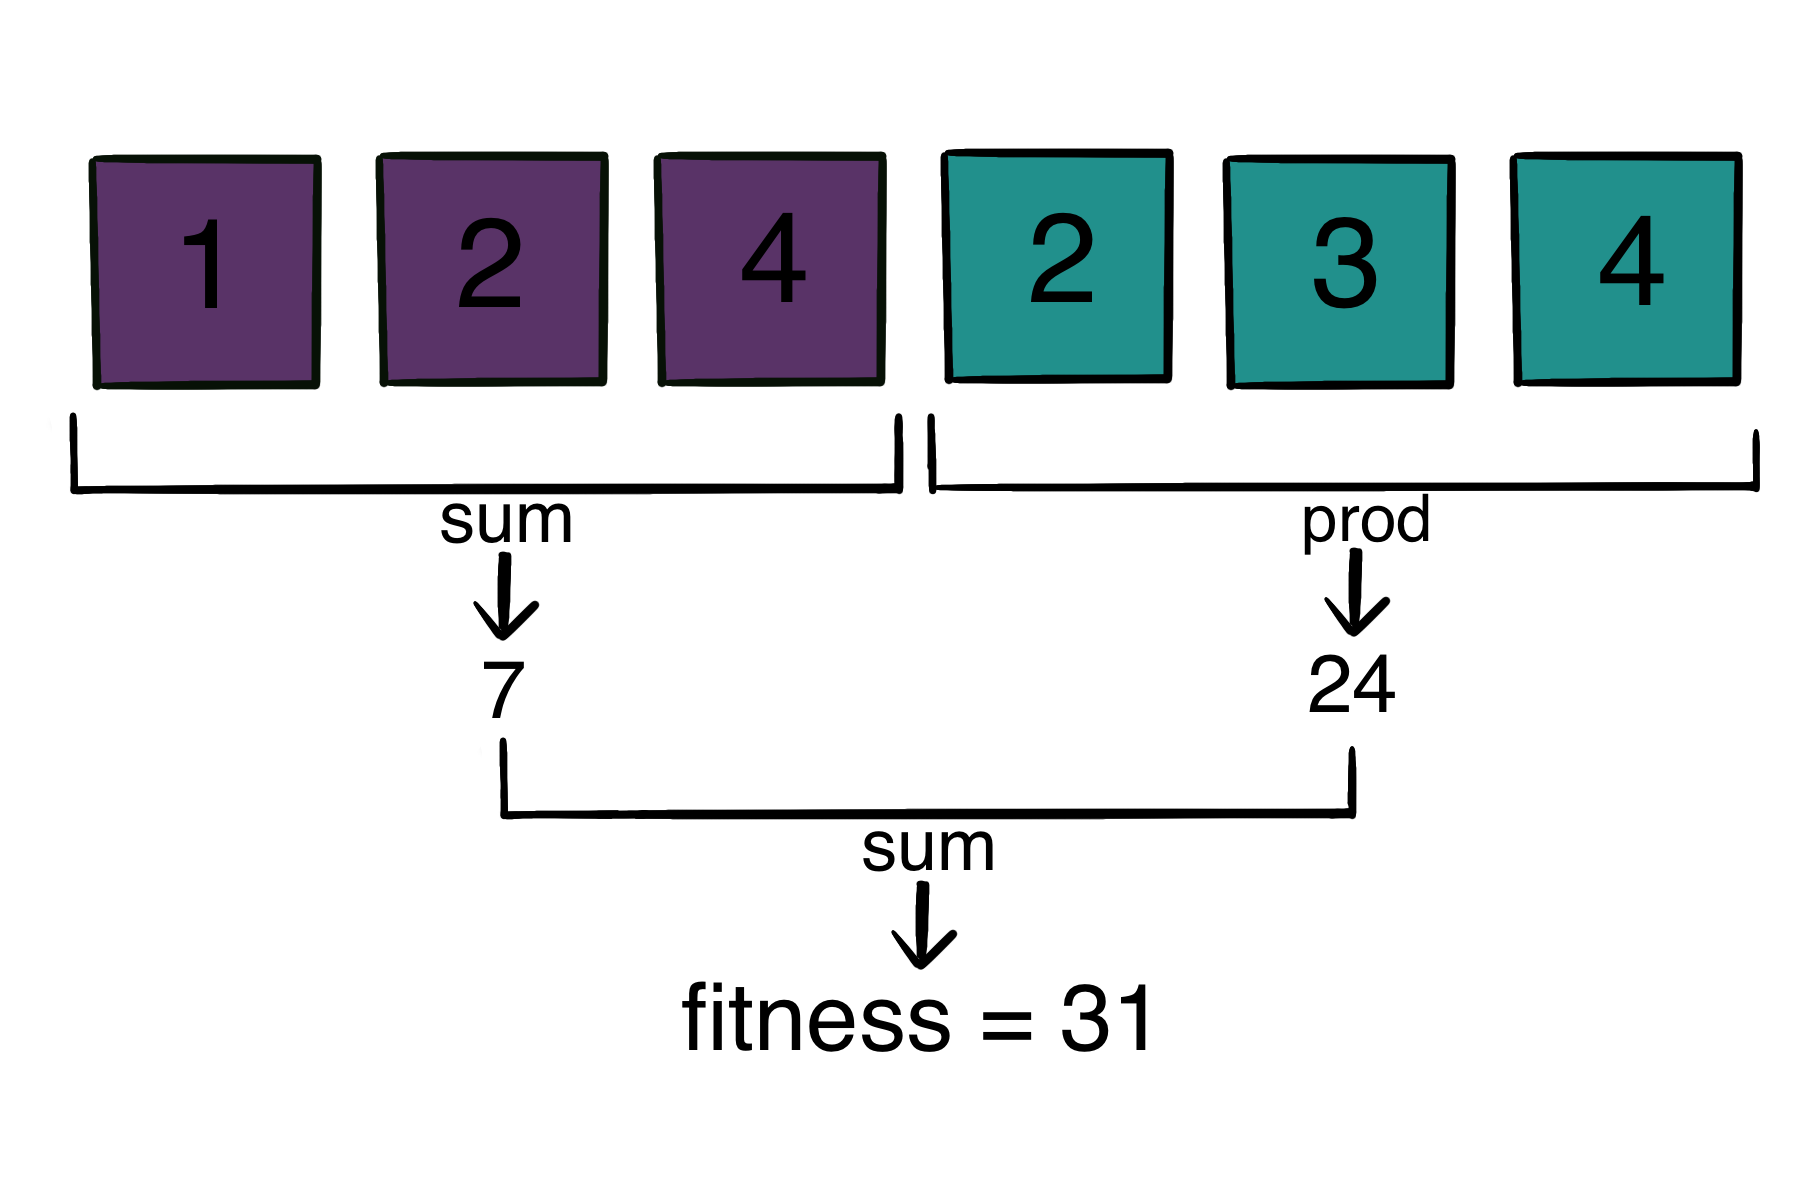
\includegraphics{chapters/1-rank-epistasis/figs/ADDMULT.PNG}}
    \caption{Schematic of additive and multiplicative genome for length $n=6$. The first $n/2$ sites are summed and the last $n/2$ sites are multiplied, then the two halves are summed for the final fitness. Image by Katie Gleason.}
    \label{fig:method:admult}
\end{figure}

In this case, the genome was a vector of length $n=20$ of integers between 1 and 4, inclusive (see Fig~\ref{fig:method:admult}). The first 10 integers are summed together, and the last 10 values are multiplied together. The total fitness is the sum of these two values. None of these sites interact epistatically; changing a single site does not affect the fitness contributions of any of the other sites. However, under a baseline assumption that sites should be additive, mutations in the sites which multiply together will appear to create a larger than expected fitness effect. The reverse is true for a baseline assumption of multiplicativity when evaluating the additive sites; they will appear to create a smaller than expected fitness effect. Therefore, we expect traditional metrics which take a baseline for the entire genome to incorrectly identify positive epistasis (under an additive model) or negative epistasis (under a multiplicative model). To determine whether rank epistasis successfully solves this problem, we compared rank epistasis with the metric $\epsilon$, which has both an additive and multiplicative form \citep{ostman_impact_2011}. 

\subsection{Identifying Degrees of Epistasis}



A good epistasis metric should be able to distinguish between different degrees of epistasis. To confirm that rank epistasis can achieve this goal, we tested it on a landscape where the true degree of interactivity at each site could be calculated.
We used Kauffman NK landscapes \citep{kauffman_towards_1987} for this purpose.
NK landscapes are commonly used epistatic models because they are \textit{tunably rugged}: in NK landscapes, \textit{N} refers to the number of sites in the genome while \textit{K} refers to the number of sites each site interacts with.
Therefore, we can tune how interactive (i.e. how epistatic) the genome is by changing the parameter $K$. 

We tested our metric on a canonical NK landscape, where all sites have equal $K$, and on two variant NK landscapes, where $K$ varied per site. 

\subsubsection{Canonical NK Landscapes}

The canonical landscape allows us to establish how the rank epistasis metric tracks known degrees of interactivity on different genomes.
Genomes in this case are bitstrings of length $N=100$.
We then allowed the population to evolve on a given NK landscape for $t=10,000$ generations and selected the most fit individual as a reference genome for the rank epistasis algorithm. 
For our canonical NK landscape, we tested the metric on values $K=0, 1, 2, 4, 8$. 

\subsubsection{Variant NK Landscapes}

The variant landscapes allow us to establish how it tracks different degrees of interactivity within the same genome.
As with the canonical landscape, genomes were bitstrings of lenth $N=100$ which evolved for $t=10,000$ generations, and the most fit individual was selected as the reference genome.
Variant landscapes were tested on all pairwise combinations of $K=0, 1, 2, 4, 8$. 

\paragraph{Variant 1: Half-and-Half}
For the first variant, which we call \textit{half-and-half}, we evaluate the first $50$ sites on one NK landscape and the last $50$ sites on a different landscape. Each landscape is independently generated. This allows us to set a different $K$ for each half of the genome. At the boundary, evaluation wraps around to the genome half with the same $K$ value; e.g., if $K=2$, site $49$ interacts with sites $0$ and $1$, whereas site $100$ interacts with sites $50$ and $51$ (Fig~\ref{fig:method:half}.

\begin{figure}
    \centering
    \fbox{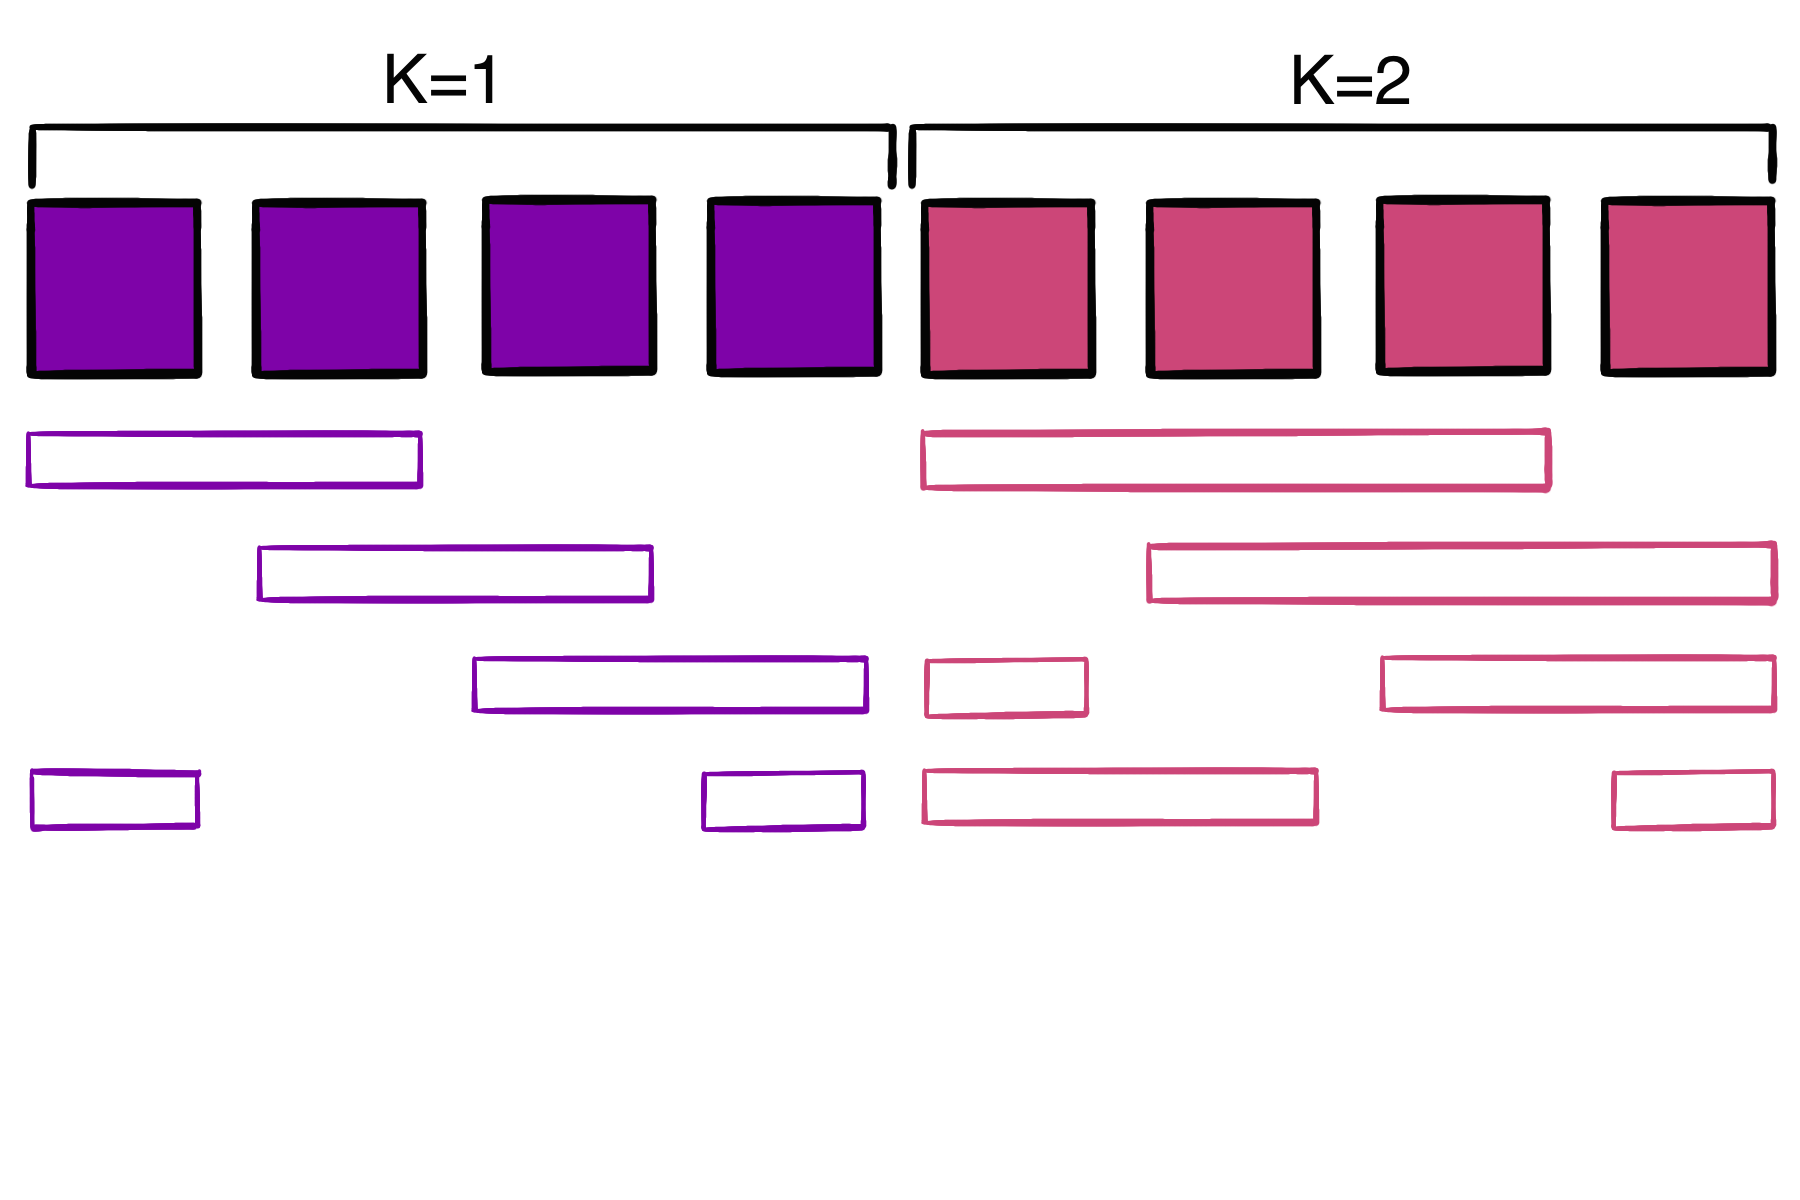
\includegraphics{chapters/1-rank-epistasis/figs/HALF.PNG}}
    \caption{Schematic for Half-and-Half landscape with first half $K=1$, second half $K=2$. Filled boxes represent sites of the genome. Empty rectangles underneath are guides for which sites are part of the same evaluation block. Image by Katie Gleason.}
    \label{fig:method:half}
\end{figure}


\paragraph{Variant 2: Mixed}
For the second variant, which we call \textit{mixed}, we evaluate odd-valued sites on one landscape and even-valued sites on a second landscape. Each site still interacts with the adjacent $K$ sites, regardless of odd or even values. In this case, evaluation wraps at the boundary of the genome rather than each landscape. As above, landscapes are independently generated.

\begin{figure}
    \centering
    \fbox{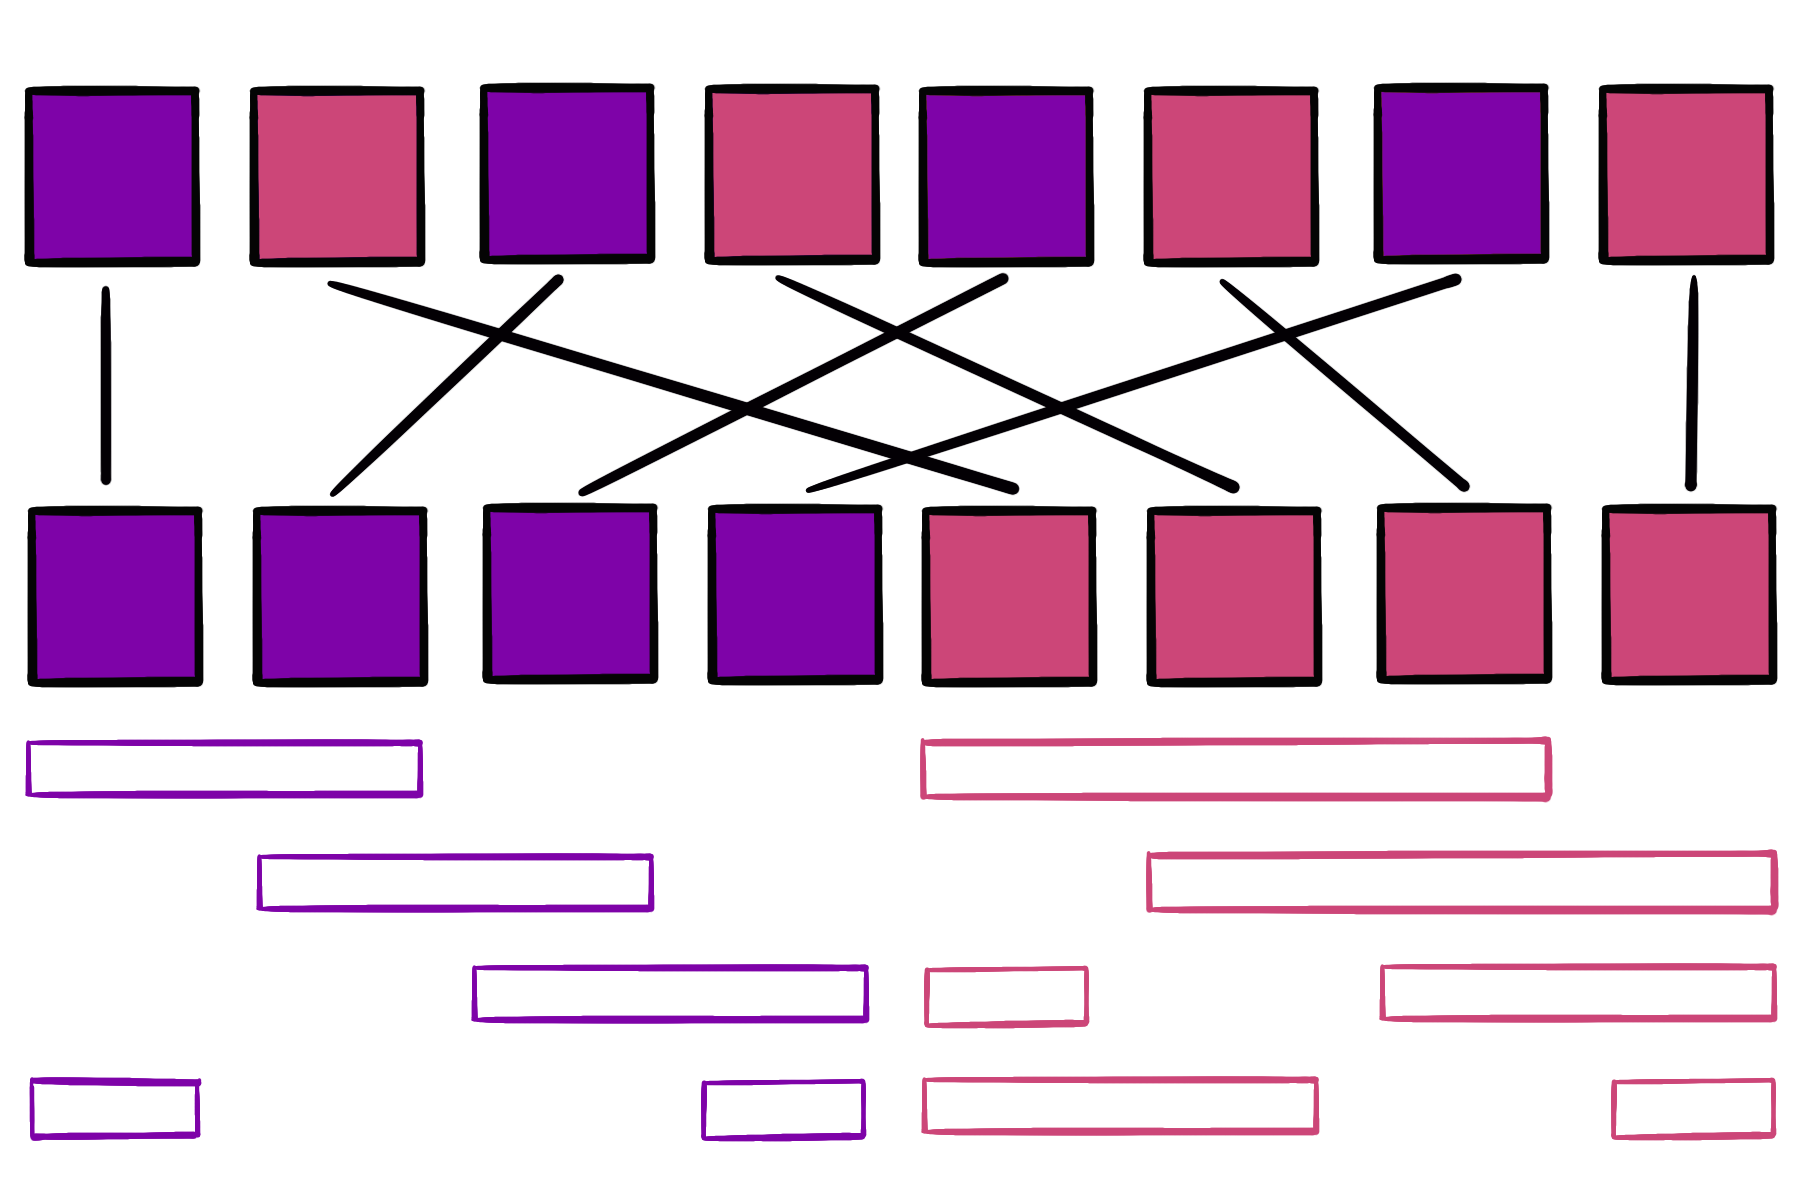
\includegraphics{chapters/1-rank-epistasis/figs/MIXED.PNG}}
    \caption{Schematic for Mixed landscape with evens $K=1$, odds $K=2$. Lines indicate how even-valued sites and odd-numbered sites are extracted to form a seperately evaluated genomes. Filled boxes represent sites of the genome. Empty rectangles underneath are guides for which sites are part of the same evaluation block. Image by Katie Gleason.}
    \label{fig:method:half}
\end{figure}


\subsection{Data and Code Availability}

Experiments on the NK landscape were conducted using the Modular Agent-Based Evolver framework (MABE2), an open-source modular digital evolution framework. The source code for MABE2 is available at \url{https://github.com/mercere99/MABE2}. Experiments for the additive and multiplicative comparison were performed in Python (v3.10.4).

Statistical analysis and data visualization was performed in R \citep{r_core_team_r_2019} with the \texttt{tidyverse} library \citep{wickham_welcome_2019}. Implementation of paired Wilcoxon is from \texttt{rstatix} \citep{kassambara_rstatix_2021}.
All data is available at \url{https://doi.org/10.5061/dryad.5dv41ns84}. 
All code for data generation, analysis, and visualization can be found at \url{https://doi.org/10.5281/zenodo.6611759}.
\section{Results and Discussion}


\subsection{Rank epistasis correctly detects no epistasis on a deceptive landscape}

We find that rank epistasis correctly detects lack of epistasis on a deceptive additive and multiplicative fitness landscape where other metrics fail (Fig~\ref{fig:res:addmult}). 

Here, the additive model detects positive epistasis, since some sites are actually multiplicative. Under its baseline assumption, the whole genome appears epistatic since the average double-mutant has a much higher fitness than expected, since some mutations are multiplied rather than summed. On the other hand, the multiplicative model detects negative epistasis, since some sites are actually additive. Under its baseline assumption, double-mutants have much lower fitness than expected, since some mutations are summed rather than multiplied.

Rank epistasis, however, correctly detects no epistasis across the entire genome. Rank epistasis does not assume additive or multiplicative interaction; it measures only relative perturbations in the rankings between single and double mutants. Without baseline assumptions, the metric is able to correctly determine that no epistasis is present in the genome, addressing a long-standing problem in detection of epistasis \citep{cordell_epistasis_2002, puniyani_meaning_2004}. 

\begin{figure}
    \centering
    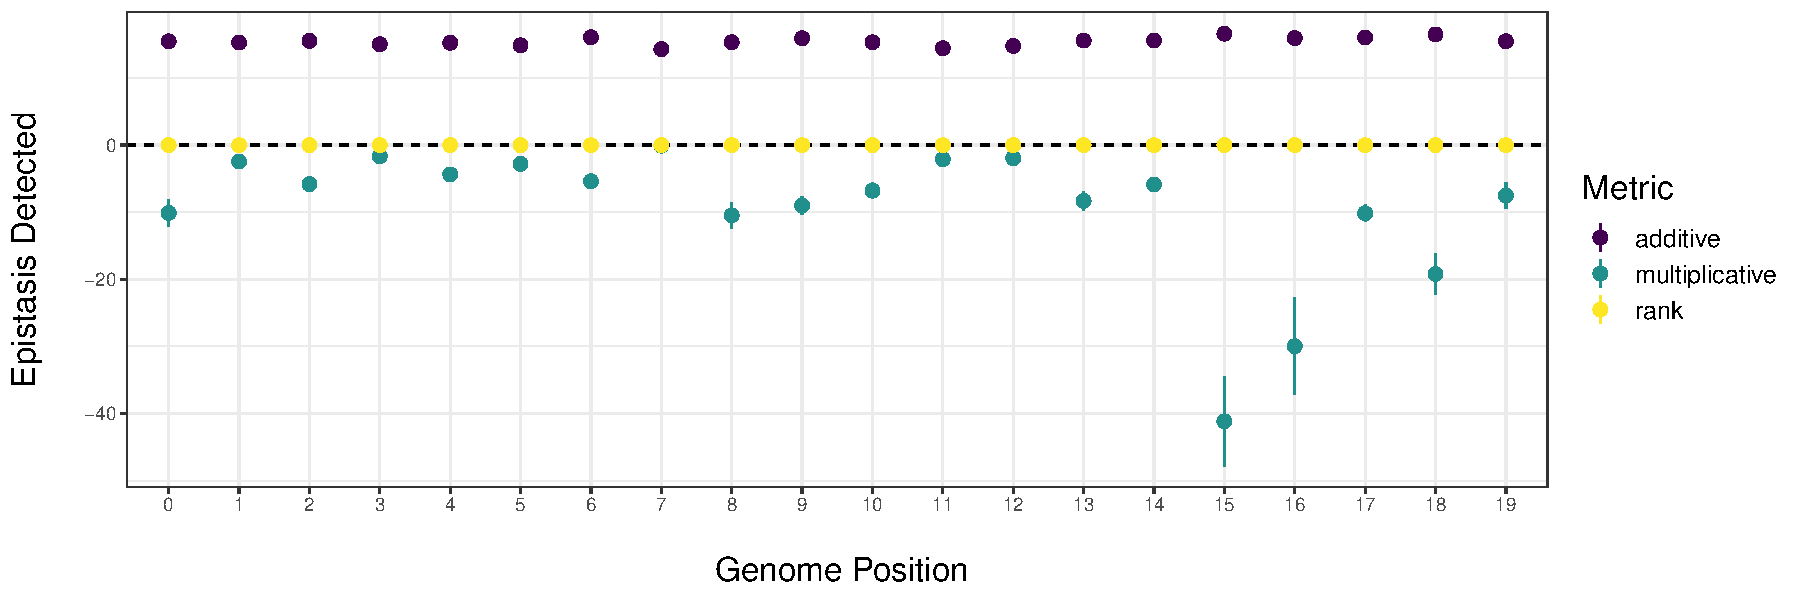
\includegraphics[width=\textwidth]{chapters/1-rank-epistasis/figs/summary_addmult.pdf}
    \caption{Comparison of rank epistasis metric to additive and multiplicative versions of metric $\epsilon$ as described in \cite{ostman_impact_2011}. Each x-axis tick represents one position in the genome, i.e., the $\epsilon$ or $\omega$ detected for that site. Note that $\epsilon$ and $\omega$ are not usually directly comparable; however, since $\omega=0$ and $\epsilon=0$ both indicate no epistasis, here $\omega$ is graphed on the same Y-axis. Dashed line at Y=0 indicates the true level of interactivity in genome. Dots represent mean and bars represent 95\% CIs for 100 replicates.}
    \label{fig:res:addmult}
\end{figure}

\subsection{Rank epistasis correlates with K on Canonical NK Landscapes}

\begin{figure}
    \centering
    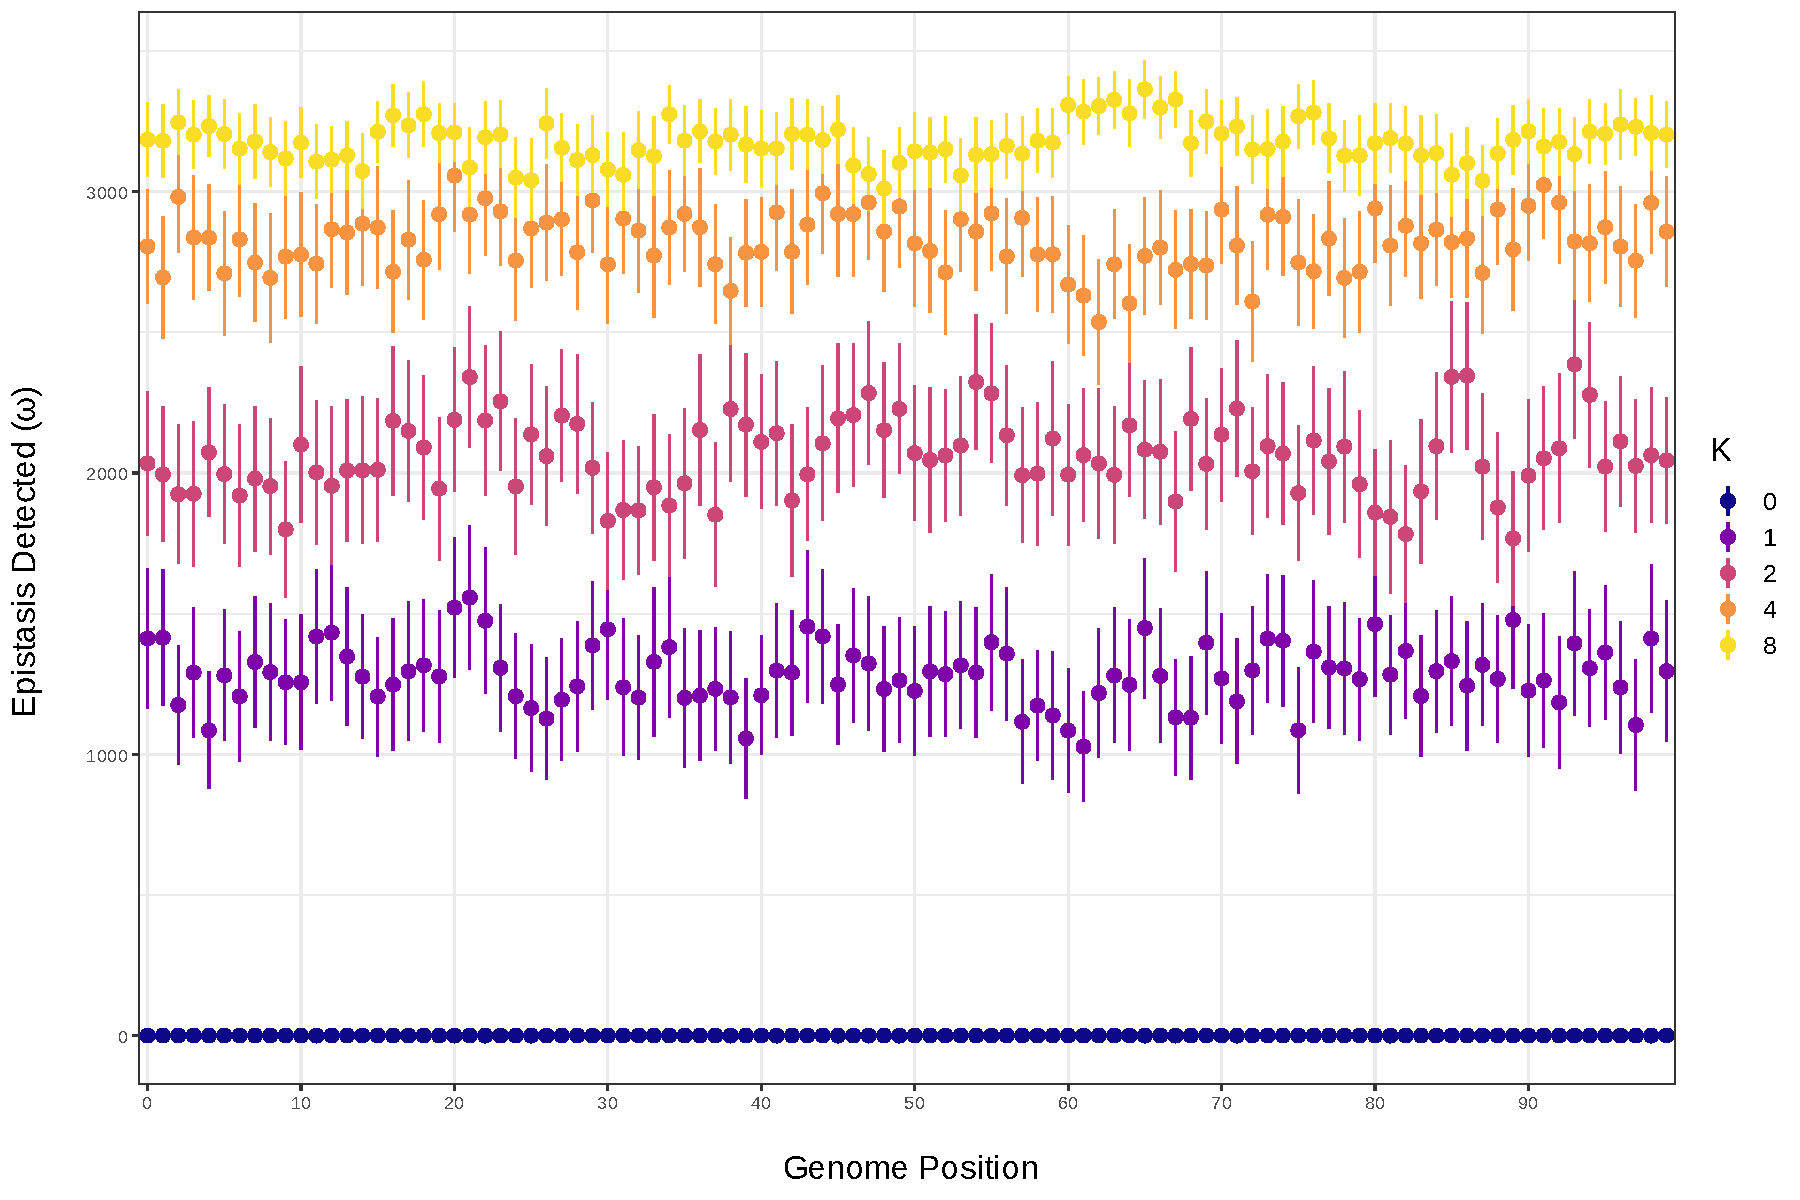
\includegraphics[width=\textwidth]{chapters/1-rank-epistasis/figs/summary_canon.pdf}
    \caption{Rank epistasis metric $\omega$ on a canonical NK landscape. Each x-axis tick represents one position in the genome, i.e., the $\omega$ detected for that site. Dots represent mean and bars represent 95\% CIs for 100 replicates.}
    \label{fig:res:canon}
\end{figure}

 On these landscapes, every site in a particular genome has the same degree of interactivity, so we expect roughly the same $\omega$ across sites. We also expect that identical landscapes with higher $K$ will generate a higher $\omega$. We find that the rank epistasis metric $\omega$ strongly correlates with $K$ when tested on traditional NK landscapes and correctly stratifies different values of $K$ when averaged across replicates (Fig.~\ref{fig:res:canon}). 

Of note is that $\omega$ and $K$ are not linearly correlated; for example, the average difference in measured $\omega$ from $K=0$ to $K=1$ is much larger than that from $K=1$ to $K=2$. In fact, as $K$ increases, the difference in $\omega$ between consecutive values of $K$ decreases.

One possible explanation for this effect is that the number of peaks in an NK landscape, and therefore the effect of perturbation on the genome, scales exponentially with $K$. In an NK landscape, each group of $K$ sites can take on $2^{K+1}$ possible fitness values. Therefore, for an NK landscape with $K=2$, each group of $K$ sites has $8$ possible fitness values, while each group in a landscape where $K=4$ has $32$ possible fitness values. NK landscapes therefore quickly reach a threshold where any mutation is likely to significantly change a genotype`s fitness; indeed, it has been shown that when $K>1$ it is exponentially difficult to find even local optima due to this effect \citep{kaznatcheev_computational_2019}.
Since rank epistasis is a measure of how perturbation affects the \textit{rank ordering} of possible mutants, genomes on NK landscapes quickly reach a point where they are close to maximally perturbed even at small $K$. This means the detected rank epistasis for $K=4$, for example, may not always be significantly different than for $K=8$ (see Fig~\ref{fig:res:canon}). Despite these limitations, on average rank epistasis is still able to distinguish low interactivity from high.

\subsection{Disentangling K on Variant NK Landscapes}

Rank epistasis successfully detects varying levels of per-site epistasis within the same genome on both variant landscapes, though the value of $\omega$ changes across genomes. In general, we find that rank epistasis on these variant landscapes produces a measure of \textit{apparent} epistasis. 

\begin{figure}
    \centering
    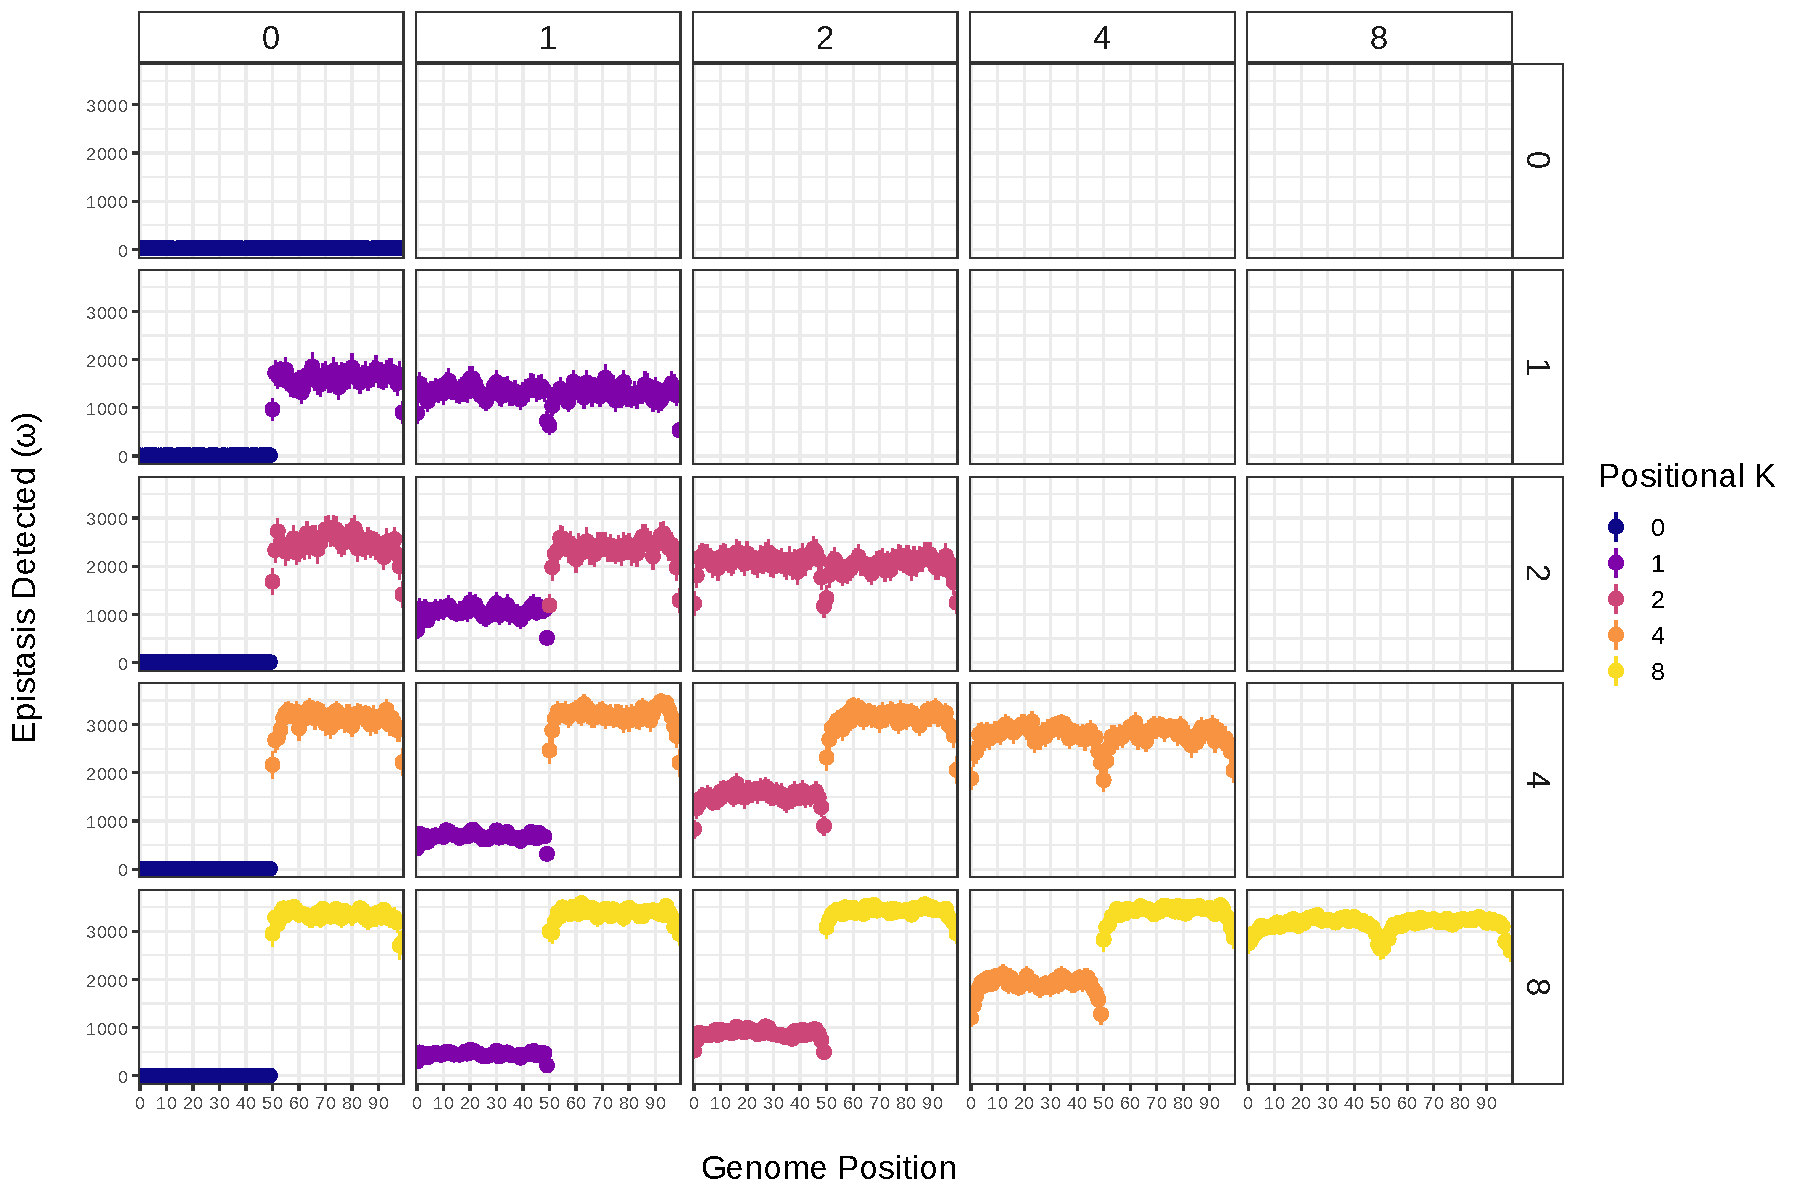
\includegraphics[width=\textwidth]{chapters/1-rank-epistasis/figs/summary_half.pdf}
    \caption{Rank epistasis metric $\omega$ on a Half-and-Half NK landscape. Top bars indicate the $K$ value set for the first $N=50$ values. Right bars indicate the $K$ value for the second $N=50$ values. Each x-axis tick within subplots represents one position in the genome, i.e., the $\omega$ detected for that site. Dots represent mean and bars represent 95\% CIs for 100 replicates.}
    \label{fig:res:half}
\end{figure}

\subsubsection{Rank epistasis measures different epistatic levels on Half-and-Half landscape}

In the Half-and-Half landscape, there is clear separation of the measured $\omega$ between the two ``halves" with different values of $K$. However, this $\omega$ is not consistently linked to values of $K$ across different landscapes. For example, the average $\omega$ for $K=4$ when $K=4$ is the higher value is around 3000, but when $K=4$ is paired with $K=8$ the $\omega$ for sites where $K=4$ is closer to 2000. However, it is still lower than the detected $\omega$ for sites where $K=8$. This result reinforces that $\omega$ represents a \textit{relative} epistatic value, rather than an absolute one. 

Additionally, on both halves of the landscape, $\omega$ appears unexpectedly lower at the boundary between halves, even for a low $K$ transitioning to higher $K$. One explanation for this effect could be that sites at the boundary are ``caught" between landscapes; since they are evolving across independent landscapes, it is difficult to find local optima on both landscapes at once. Therefore, the genomes may evolve to be more robust to mutation around these sites, finding lower fitness regions where mutations do not cause high perturbation of fitness and therefore where $\omega$ measures at lower than surrounding sites. This phenomenon, termed ``survival of the flattest", is well-documented in the literature \citep{wilke_evolution_2001, franklin_mapping_2019}. This observation suggests that rank epistasis may identify interesting features of genetic architrecture beyond interactivity, such as evolved mutational robustness.

\subsubsection{Rank epistasis measures apparent epistasis on Mixed landscape}

\begin{figure}
    \centering
    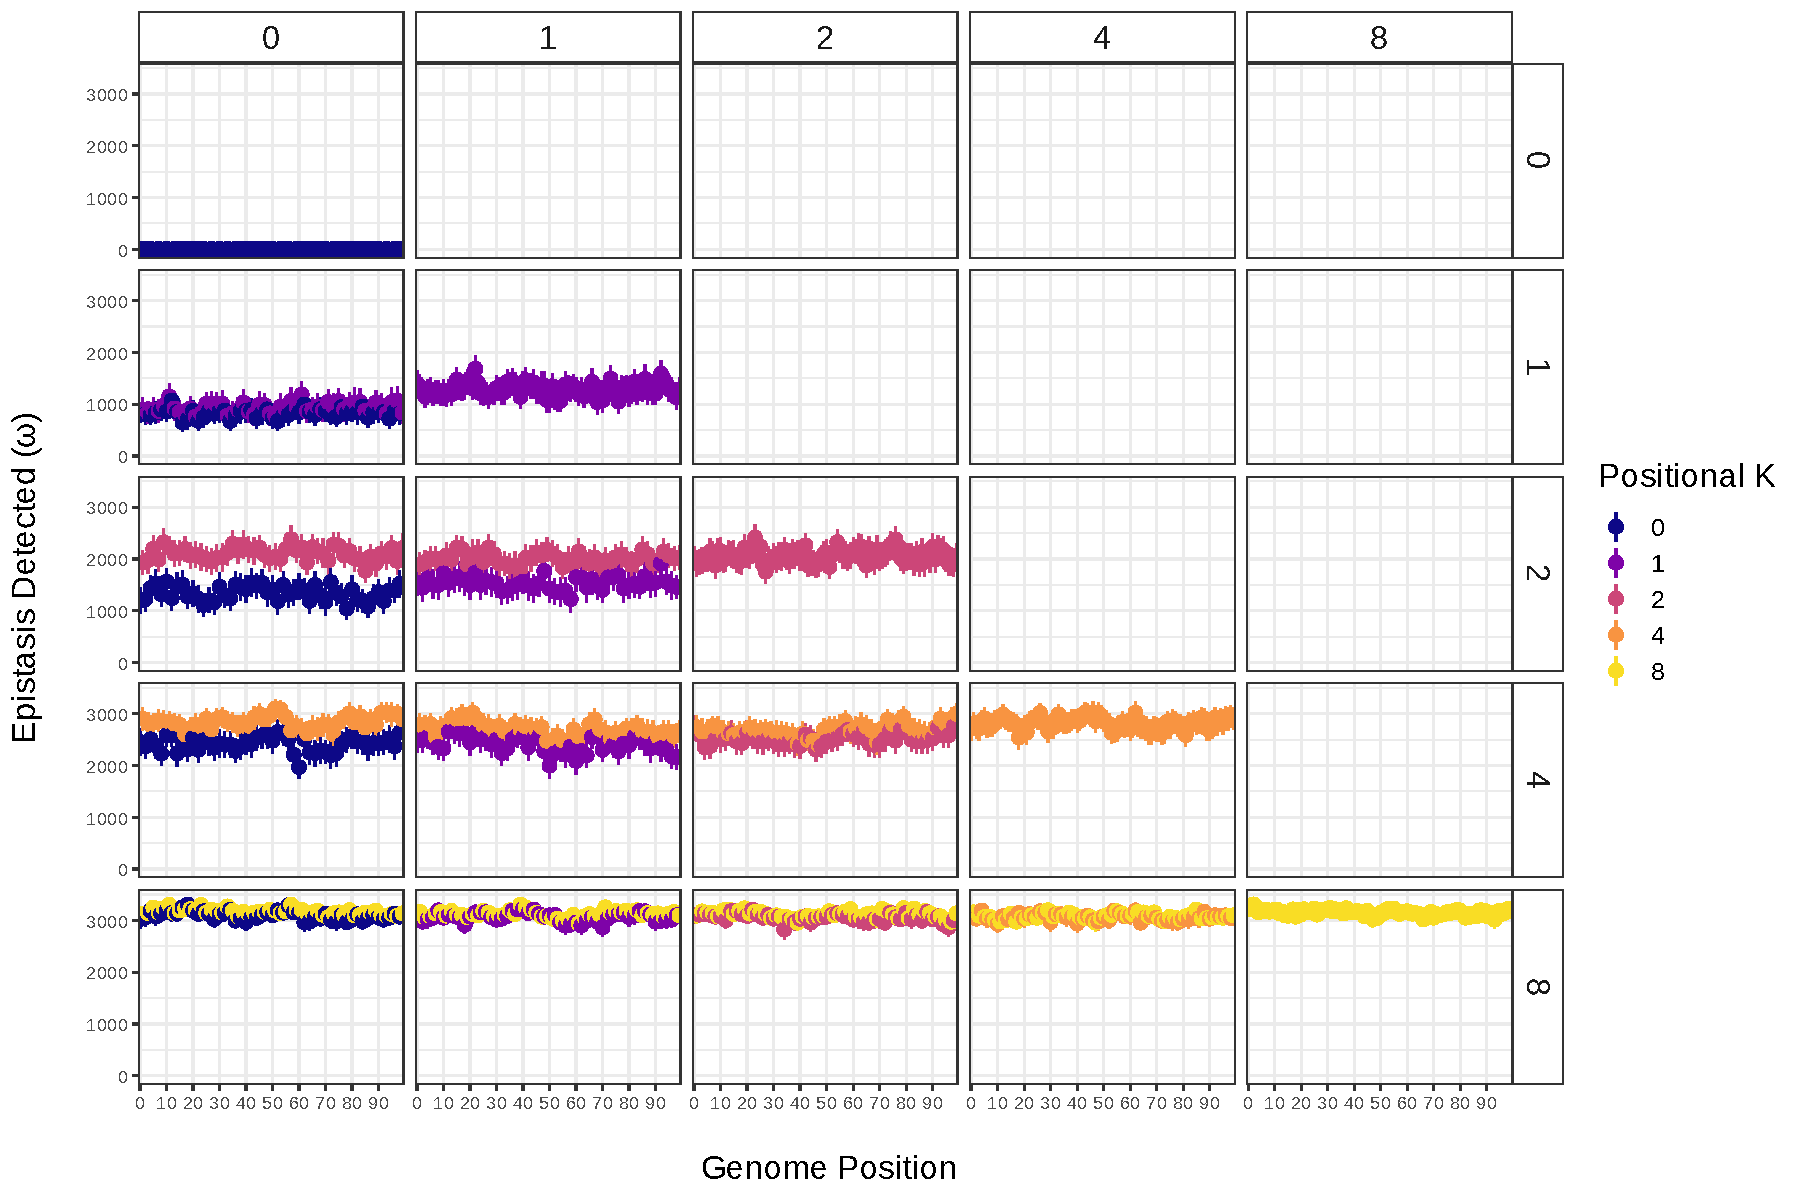
\includegraphics[width=\textwidth]{chapters/1-rank-epistasis/figs/summary_mixed.pdf}
    \caption{Rank epistasis metric $\omega$ on a mixed NK landscape. Top bars indicate the $K$ value set for even-valued. Right bars indicate the $K$ value for odd-valued sites. Each x-axis tick within subplots represents one position in the genome, i.e., the $\omega$ detected for that site. Dots represent mean and bars represent 95\% CIs for 100 replicates.}
    \label{fig:res:mixed}
\end{figure}

In the Mixed landscape, separation of $K$ values is less clear. As the higher $K$ increases, the difference in $\omega$ between lower and higher $K$ values generally decreases; one exception is in the comparison of the mixed $K=0/K=1$ landscape vs. $K=0/K=2$ landscape (Fig~\ref{fig:res:mixed}). 

It is likely that the overall effect of reduced separation of $\omega$ is due to a similar effect as described in the results for the canonical landscape; since evaluation takes place across multiple landscapes, the highly rugged landscapes for large $K$ dominates the level of perturbation detected. In fact, $\omega$ here can be seen as a measure of the ``true" $K$ for each site, as odd- and even-valued sites are \textit{evaluated} on landscapes of different values for $K$ but \textit{interact} with the same number of adjacent sites due to overlap. 

This measurement of ``true $K$" also explains the behavior in the landscapes with $K=0/K=1$ compared to $K=0/K=2$. In the former case, each site where $K=1$ directly interacts with a site where $K=0$, bringing the true interactivity of every site to $K=1$. In the latter case, evaluating every other site with $K=2$ causes the $K=0$ sites to fall completely inside the evaluation block, and interact with only one of the $K=2$ sites at a time. In higher $K$ the landscape staggering does not match the size of the evaluation block and the effect is lost.

\section{Conclusion}

Rank epistasis is a promising new metric to detect interactivity at specific sites in a genome without the need for a baseline assumption of additivity or multiplicativity; therefore, unlike existing metrics, there is no risk of selecting the wrong baseline assumption and falsely detecting epistatic activity where there is none. Additionally, rank epistasis is able to accurately detect a lack of epistasis when both additive and multiplicative baseline interactions are present, which existing metrics are unable to account for. The metric is also able to reveal areas of high mutational robustness within a genome.

One major difference between rank epistasis and existing metrics is that it does not give an indication of \textit{positive} or \textit{negative} epistasis, only the \textit{degree} of epistasis and how much perturbation is present in the ordering of possible mutants. Other metrics may be more appropriate if the sign of epistasis is of particular interest; however, if detection of site interaction and the overall density of the mutational landscape is the primary goal, rank epistasis can be a strong choice of metric. Additionally, it can be used to supplement sign epistasis metrics to ensure the measured epistasis is not an artefact of baseline assumptions.

 Here we do not provide biological applications for rank epistasis as it is beyond the scope of this paper. However, this metric could be easily applied to any sufficiently complete biological dataset in the same way it is applied here to computational ones. It is our hope that using rank epistasis in this way to detect genome connectivity in biological systems will lead to a fuller understanding of the complex ways in which genome structure dictates function.
\section*{Author Contribution Statement}

All authors drafted and edited this paper. ALA wrote the code, conducted the experiments, and analyzed and interpreted the results. ELD and CO provided theoretical guidance. CO conceived of the original idea for the study.
\section*{Acknowledgements}

The authors thank Christoph Adami, Wolfgang Banzhaf, Austin Ferguson, and Connor Grady for assistance on the design of this study. The authors also thank artist Kathleen (Katie) Gleason for her contributions to the figures.
This material is based in part upon work supported by the National Science Foundation under Cooperative Agreement No. DBI-0939454 
and by a National Science Foundation Graduate Research Fellowship to ALA. 
Any opinions, findings, and conclusions or recommendations expressed in this material are those of the author(s) and do not necessarily reflect the views of the National Science Foundation.
This work was conducted on the ancestral, traditional and contemporary lands of the Anishinaabeg – Three Fires Confederacy of Ojibwe, Odawa and Potawatomi peoples.

\chapter{The comparative hybrid approach to investigate cognition across substrates}
\label{ch:chm}

\noindent Authors: Sarah Albani*, Acacia L. Ackles, Charles Ofria, and Clifford Bohm \\
This chapter is adapted from \cite{albani_comparative_2021}, which underwent peer review and appeared in the proceedings of the 2021 Artificial Life Conference.\\
* Undergraduate Author

\section{Introduction}

The concept of cognition is a subject of study in both neuroscience and artificial intelligence.
Studying cognition can lead to a greater theoretical understanding of what allows cognitive processes to function, as well as an understanding of how to harness these processes for problem-solving.
Much of machine learning was inspired by the effective mechanisms found in natural systems, which may explain many of their functional similarities.
However, while natural brains are effective at producing robust forms of general cognition, human-designed digital structures have not yet demonstrated general intelligence. 
On the one hand, it may be that we have not gained a sufficient understanding of biological intelligence to implement it in silico. 
On the other hand, perhaps modern computer systems simply lack some fundamental properties (such as massive parallelism) which make a direct implementation of a biological algorithm for intelligence infeasible. 
There are a number of disparate approaches to AI based different understandings of biological systems (e.g.~ANN \citep{rosenblatt_perceptron_1958}, HTM \citep{hawkins_hierarchical_2011}, spiking neural nets \citep{ghosh-dastidar_spiking_2009}) or built up from mathematical or logical foundations (e.g.~Avida \citep{ofria_avida_2004}, Markov Brains \citep{hintze_markov_2017}, Signal GP \citep{lalejini_evolving_2018}, Tangled Program Graphs \citep{kelly_multi-task_2017}). 
A real problem in the field is an inability to directly compare these various systems and to draw concussions across the various approaches. 
This makes can make it difficult apply discoveries in one area of AI research to others and to relate research results from AI and neuroscience.
Therefore, from an Artificial Life perspective, we want to expand beyond biomimetic approaches to producing machine intelligence and move towards a more holistic view that includes the underlying evolutionary processes that produced general cognition in nature.

Evolution took billions of years to produce agents that engage in intelligent behavior; we would prefer not to wait that long.
While evolution in natural systems is driven by an underlying stochastic process, we are not restricted by the rate of random occurrences of beneficial mutations. 
We can take a more directed approach by systematically studying the evolution of cognition in digital systems. 
Ideally, we want to provide hands-on guidance to produce AI in a much shorter time, while simultaneously harnessing the creative and constructive potential of evolution to allow our digital systems to reach their full utility.  
To bootstrap this process, we must conduct a systematic study of potential evolutionary building blocks and underlying representations that are both computationally efficient and effective for evolving cognition.

Previous work has often compared whole neural architectures' performance on a particular task of interest.
For example, algorithm performance has been studied in detail on tasks such as general classification \citep{williams_preliminary_2006,singh_review_2016, binkhonain_review_2019}, text recognition \citep{khan_review_2019}, disease prediction \citep{uddin_comparing_2019}, and ecological modeling \citep{crisci_review_2012}, to name a few.
However, due to the numerous details related to design and parameterization of any particular structure, performance comparisons can not necessarily reveal why one structure outperforms another, nor investigate how their component parts may account for the results. 

Some work, particularly in algorithm optimization, has dealt with combining components of multiple structures to create efficient computational hybrids.
One such technique is the ``Buffet Method", which allows a computational structure to access an array of different types of information processing sub-structures during the evolutionary process\citep{hintze_evolutionary_2019} and shows that the proportion of sub-structures used in the evolved solutions is task dependent. 
Another method known as ``Auto ML" is designed to evolve a substrate from basic mathematical principles \citep{real_automl-zero_2020}. 
While these methods have been successful in optimizing task performance, they rarely look ``under the hood" at the exact variables responsible for cognitive success.

Our goal here is to demonstrate an approach for comparing cognitive substrates that allows us to identify which aspects of each substrate confer strengths in evolving solutions to cognitive processing tasks.
Here, ``substrate" refers to the virtual hardware underlying each digital representation---that is, the stuff from which each model of cognition is built. 
This concept of comparing two brains by testing hybrids based on these differences is what we have termed the \textit{Comparative Hybrid Approach}. 
In this approach, we first identify the minimal number of differences between each substrate and then develop hybrid versions which represent intermediate forms. 
These are evaluated on different cognitive tasks in order to determine if some of the identified differences can account for performance variance.
While our current focus is on only two such systems, a wider application of this approach will allow us to isolate properties of different types of components across more substrates and ultimately provide clearer guidance for designing new types of evolvable cognition.

This method is similar to knock out experiments in biology, where some aspect of a system is disabled and tests are conducted to identify changes to the system's response as a whole.

The conceptual backing for this method could be extended to more complex systems, from comparisons between more divergent digital structures to, simulations of accurate biologically-based models, or even actual biological systems (although this would require the ability to manipulate biological structures in a controlled manner).

In this work we compare Markov Brains and Recurrent Artificial Neural Networks (RNNs). 
In particular we identify differences in the logic that each brain has access to, how the logic units are connected (sparsity), and how memories are stored (discretization). 
We find that, while we observed performance differences on each axis of change, discretization in particular was the strongest indicator of task performance.
\section{Methods}

\subsection{MABE: Modular Agent-Based Evolver}

For the experiments in this work we used MABE, the Modular Agent Based Evolver framework \citep{bohm_mabe_2017}. 
We have configured MABE so that agents have a \textbf{genome} (a collection of heritable and mutable data) and a \textbf{brain} (a computational structure that receives input and generates output) specified by the genome. 
MABE manages the evolution of populations of agents by repeatedly evaluating agents in \textbf{worlds} (a fitness-bearing task) and using the results to select parents whose mutated offspring make up future generations. 
The advantage of the MABE framework is that the brains and worlds are completely modularized and therefore can be easily exchanged without altering other system properties, allowing for fast, direct comparisons. 
This ``plug-and-play" feature makes MABE well suited to not only our current cross-brain and cross-world examination, but also to the proposed future extensions of this work.

\subsection{Brains: RNNs and Markov Brains}

In MABE, a brain is a process that converts a list of values \textit{$T_0$} to a new list of values \textit{$T_1$} (Fig~\ref{fig:brains}A). 
We define the $T_0$ values as inputs (i.e. sensor readings or the state of the task) combined with the brain's memory and we define the $T_1$ values as outputs (i.e. values that determine behavior) combined with new memory values (which will be provided to the brain on the next update). 
Each time we want the brain to act (i.e. ask the brain ``what will you do now?") we set the $T_0$ values, allow the brain to run its internal process, and read the resulting $T_1$ values. 

For this work, we compare two well-studied computational structures: RNNs and Markov Brains. 
These structures can be implemented in a number of ways; we describe here our particular implementations. 
It is important to note that these particular implementations are designed not for speed of computation, but for ease of structural analysis.

In all of the experiments described in this work, both the RNNs and Markov Brains have eight memory values.

\begin{figure*}
    \centering
    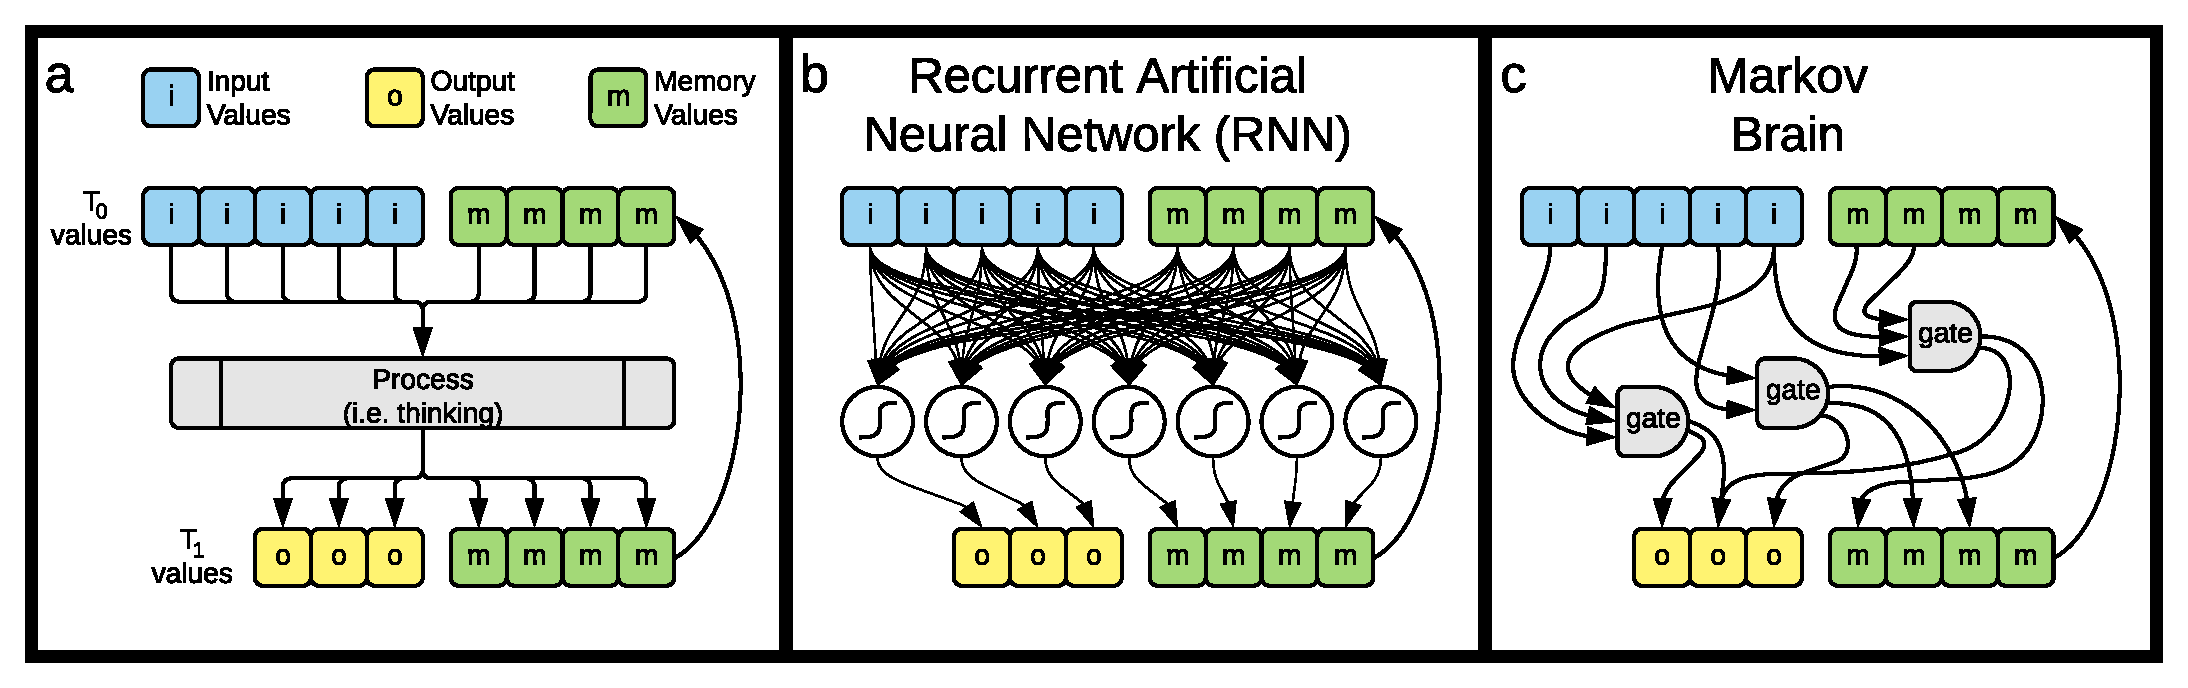
\includegraphics[width=\textwidth]{chapters/2-comp-hybrid/figs/ALIFE_2021_SI_Brains.pdf}
    \caption{Schematics showing structures of A) a generic brain, B) an Recurrent Artificial Neural Network (RNN) and C) a Markov Brain.}
    \label{fig:brains}
\end{figure*}

\subsubsection {Recurrent Artificial Neural Networks:}
RNNs are a well-studied digital neural architecture; see \cite{yu_review_2019} for a review focused on RNNs and learning. 
Typically, RNNs are used in consort with back propagation or other machine learning methods; here, we are instead using neuroevolution. 
In our particular implementation, the internal structure of the RNN (Fig~\ref{fig:brains}B) is a  list of nodes, with one node for each  $T_1$ value. 
Each node has a bias, and a weight for each $T_0$ value. 
When the RNN updates, each node adds its bias to the summation of the product of each $T_0$ value and its node-specific weight for that value, and applies $\tanh$ (a sigmoid function) to the result (which maps the value to the continuous range $\left[ -1,1 \right]$). 
The resulting values are assigned to their respective output and memory values. 
The genome is used to determine the node weights and biases via a direct encoding.

\subsubsection{Markov Brains:}
Markov Brains are a relatively new computational structure that have shown promise in studying evolution of learning \citep{hintze_markov_2017, edlund_integrated_2011, sheneman_evolving_2017}. 
The internal structure in the Markov Brains (fig:\ref{fig:brains}C) consists of wires and gates. 
Markov Brains have been studied with a number of gate types, but here we used gates with binary lookup tables that have from 2 to 4 in-wires and 2 to 4 out-wires. 
In-wires connect $T_0$ values to gates and out-wires connect gates to $T_1$ values. 
When the Markov Brain updates, each gate uses its lookup table to convert input wire values to output values. 
Each $T_1$ value is the sum of the values provided by the output wires connected to it.
An indirect encoding method is used to convert genome values into gates. 
Gates are defined by a ``start codon" (a specific set of genome values) with the following values determining number of inputs, number of outputs, the wiring of inputs and outputs, and the lookup table.

\subsubsection{Comparison of Brains}

Using the definition of the two brains, Markov Brains and RNNs, we can, in three steps, alter the description of the Markov Brain to that of the RNN, or visa versa.

Two of the alterations involve the internal processing and wiring of the brain. 
To alter the definition of a Markov Brain to that of an RNN we would first change the data processing unit from binary lookup table gates to summation and threshold nodes. 
Then, we would trade out the sparse wiring of the Markov brain for the fixed fully connected weighted wiring of the RNN.
This identifies two obvious differences inherent to the internal architectures: the method of data processing and sparse vs dense connectivity.

The third required change relates not strictly to the internal architecture, but to the potential range of memory values. 
The binary lookup table gates in Markov brains are limited to binary values, while RNNs are able to operate on continuous value ranges. 
As a result, the 8 binary (i.e. discrete) memory values in the Markov Brain represent a much smaller set of possible states than the 8 continuous range memory values in the RNN. 
In fact, the third change---changing memory from discrete to continuous---is implicit and automatic, as the summation and threshold nodes operate on continuous value ranges.

\begin{figure}
    \centering
    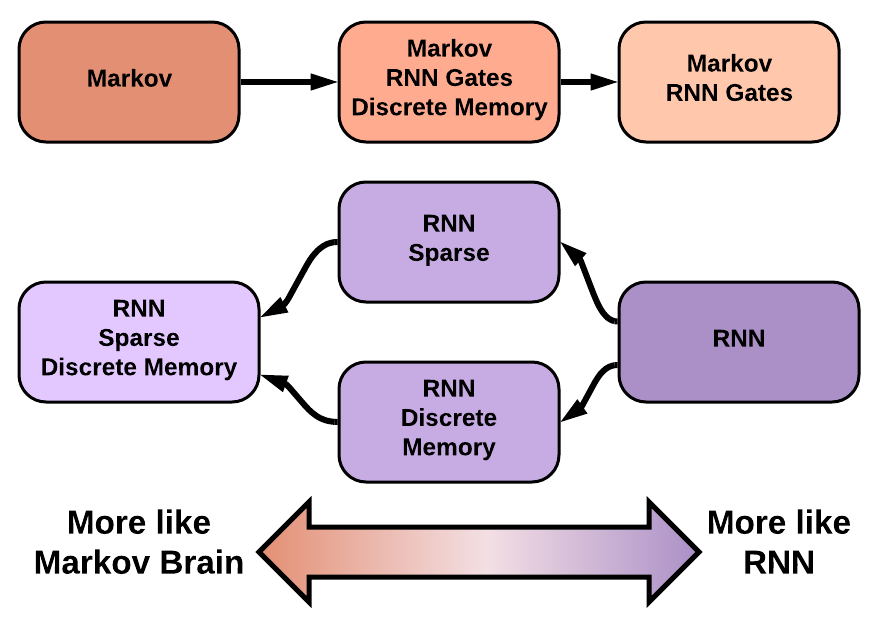
\includegraphics[width=0.4\textwidth]{chapters/2-comp-hybrid/figs/Markov_vs_RNN_H.png}
    \caption{Schematic of hybrids. Orange (top) are Markov-based; purple (bottom) are RNN-based. Arrows indicate a single change away from the canonical brain structure.}
    \label{fig:hybrids}
\end{figure}

\subsubsection{Hybrid Brains}

We implemented a number of features in RNNs and Markov Brains to allow us to create ``hybrid" brains based on each brain type (see Fig~\ref{fig:hybrids}). 
These hybrids are representative of the architectural changes described above which theoretically transform one brain type into the other, and allow us to make those changes in a step-wise fashion, one change at a time.

For Markov brains, we implemented an RNN gate that can stand in place of the canonical lookup table gate. 
These gates have the same node summation and threshold properties as the RNNs. 
The wiring of the RNN gates is sparse and determined by the same genetic encoding as the lookup table gates with the exception that these gates have from 1 to 8 inputs and a single output. 
This replacement constitutes the change to the logical operator described above. 
To approximate the difference in the range of memory values, we added a setting so that memory is either bitted (i.e. mapped to binary such that values of 0 or less are set to 0 and values greater then 0 are set to 1) as in canonical Markov brains, or continuous as in canonical RNNs. 
These changes allow us to test three Markov-based brain variants: a canonical Markov Brain, a Markov-RNN hybrid with discrete memory (i.e. RNN gate with bitted memory), and a Markov-RNN hybrid with continuous memory (i.e. RNN gate without bitted memory). 

In RNN brains, we directly varied the sparsity of their wiring and the discretization of memory. 
To implement sparsity, we biased the genome conversion so that wires with weight 0 were as common as wires with non-zero values. 
This meant that the inital population of randomly generated sparse brains would have on average half as many active connections as fully connected brains. 
As this ratio was only established at initialization, and not enforced thereafter, it could change as a result of evolution. 
To implement the discretization of memory, we added a bitting setting as in the Markov Brains. 
We tested four RNN variants: a canonical RNN, a sparse RNN (i.e. biased weights), a discretized RNN (i.e. bitted memory), and a sparse and discretized RNN (i.e. both biased weights and bitted memory).

\subsection{Worlds}

\begin{figure*}
    \centering
    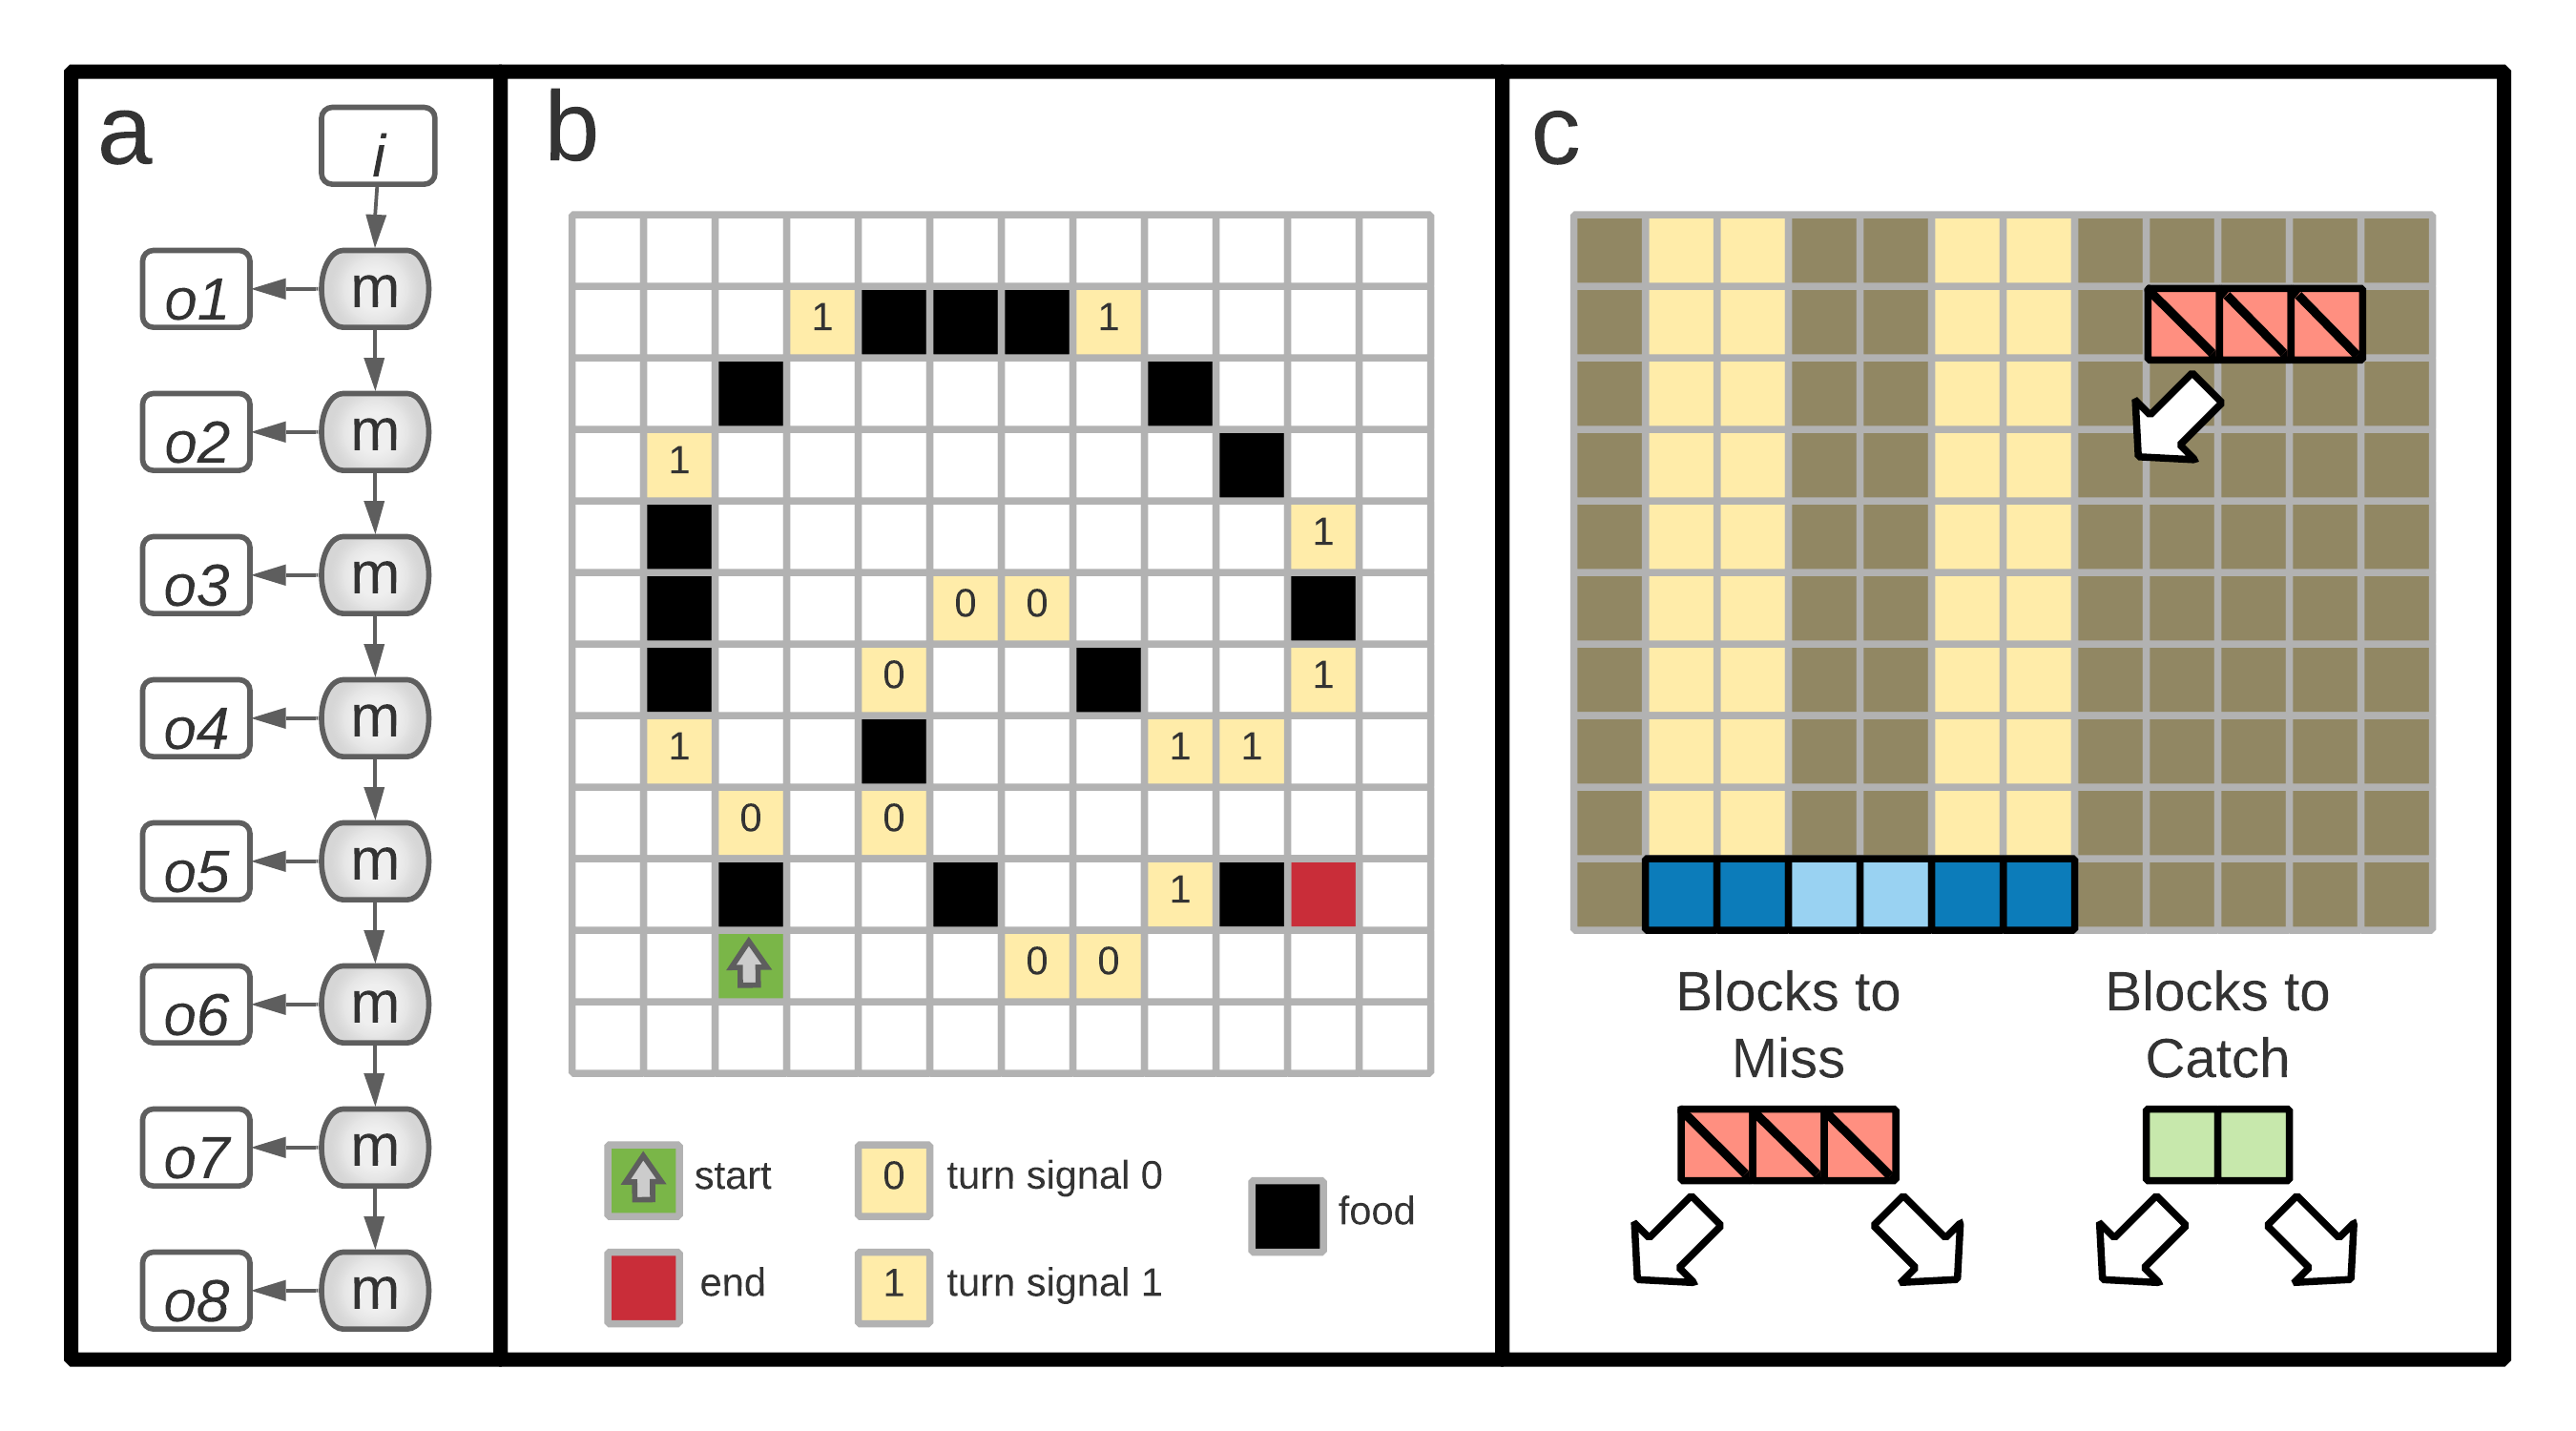
\includegraphics[width=4.5in]{chapters/2-comp-hybrid/figs/ALIFE_2021_SI_Worlds.png}
    \caption{Depictions of the worlds on which the brains were evolved. (A) \textbf{NBack.} Visualization of the data flow required to perform the NBack 8 task of recalling the previous 8 given bits. Here $i$ represents input, $m$ represents memory, and $o1$ through $o8$ represent outputs. (B) \textbf{PathFollow.} Example map from the PathFollow task. Agents start on the green start square facing in the direction of the path. Black indicates path locations with food, where the agent must move forward and which the agent is rewarded for visiting. Yellow indicates locations with randomized turn signals which the agent must associate with either left of right turn. Red indicates the end of the path. Agents that reach the end of the path receive an additional reward if they have visited all "food" locations. (C) \textbf{BlockCatch.} Spatial layout of the BlockCatch task. Blue indicates the agent; dark blue indicates the location of the sensors. Bright yellow indicates the area visible to the sensors, while darker yellow indicates area that is not visible in the agent's current location. Green (blank) and red (hatched) depict blocks that should be caught or missed and arrows indicate possible lateral motion of blocks as they fall.}
    \label{fig:worlds}
\end{figure*}

Since our work is motivated by understanding learning in the context of computational architectures, we tested each of our hybrid brains on three learning-based tasks with diverse characteristics. 
One task dealt primarily with short term memory (NBack), the second with simple information integration and lifetime memory (PathFollow), and the third with more complex information integration and lifetime memory (BlockCatch). 
We provide an in-depth analysis of the required logic and information integration required for each task and thoughts about how this relates to the results in the Discussion section titled Information Integration.

%To test the brains we evolved each brain type in three worlds (i.e. tasks or environments).

\subsubsection{NBack World}
NBack world (Fig~\ref{fig:worlds}) presents a simple short-term memory task. 
In this task, agents are presented a bit stream, one bit at a time, and must respond with the last 8 bits they were provided. 
We tested each agent 10 times with 18 inputs presented per test. 
Only the outputs associated with the last 10 inputs were evaluated. 
Agents received a score based on the ratio of the correct outputs to the total number of outputs.
NBack is based on a common cognitive task in neuropsychology to test working memory via neuroimaging, though its efficacy in human subjects is under review \citep{owen_n-back_2005, miller_is_2009, jaeggi_concurrent_2010}.

\subsubsection{PathFollow World}
In PathFollow world (Fig~\ref{fig:worlds}B), agents must learn to respond to a variable environmental clue. 
Agents exist on a grid and are able to sense symbols only on the space they are currently occupying. 
Agents must use those symbols to navigate a path defined by food and randomized turn signals. 
Agents can move forward and backwards, and turn left and right 45 degrees. 
Each location in the world contains a symbol that marks that location either as start, end, empty, food, turn signal 0, or turn signal 1. 
Agents start on the start location oriented towards the next step on the path. 
Visting a food location provides reward (used to determine reproductive success) and indicates a continuation of the path. 
If the agent steps off the path they receive a small penalty. 
The two turn signals indicate turns in the path, but these signals' meaning are reset every time an agent starts a new path. 
That is, signal 0 may indicate a left turn or a right turn, and signal 1 will indicate the opposite of the direction of signal 0. 
In order to perform well in Path Follow world, agents must form an association between the turn signals and their meaning by trial and error, and then must remember these associations for the remainder of that path.
Agents are scored on their ability to reach the end of the path while visiting all locations and minimizing time off the path.
PathFollow world is a simplified version of the task presented in \cite{pontes_evolutionary_2020}; in the previous work, the turn signals were not restricted to a binary choice.

\subsubsection{BlockCatch World}
BlockCatch world (Fig~\ref{fig:worlds}C) is a task that requires both lifetime memory and complex information integration. 
Agents are rewarded based on whether they catch or avoid a block that falls towards them \citep{marstaller_evolution_2013}. 
The world is a $20 \times 20$ grid, and agents are paddles that move left and right at the bottom of the world. 
Agents are 6 units wide and have 4 sensors that look up and can detect if there is an object directly above them, but not the distance to the object. 
The sensors are positioned such that the agent has a 2 unit wide blind spot over its center. 
Blocks of either size 2 or 3 begin at the top of the world and fall toward the agent one at a time. 
The blocks fall by moving horizontally one space, either left or right, and vertically down one space at a time. 
If a block is size 2 the agent should "catch" the block (i.e. be positioned such that block intersects some part of the agent when the block has fallen to the level of the agent), and if a block is size 3 the agent should "miss" the block. 
Agents must integrate sensor input over time both to determine the block shape (to decide whether to catch or avoid) and the direction the block is moving (to correctly position themselves). 
They therefore must also remember the block size and direction once they have detected these features and behave accordingly. 
Agents are tested on every combination of block size and direction and receive a score that is the ratio of correct results over all tests.

\subsubsection{Experiment Details}
Each described brain variant was evolved on each described world 100 times (i.e. 100 replicates of each experiment) for 200,000 generations.
In all cases, we used populations of 100 agents and tournament selection (size 5). 
Agents' genomes were vectors of integer values in the range [0,255] with initial length 5,000. On reproduction, offsprings' genomes could be altered by insertion and deletion mutations of size 128 to 512 at a per site rate of 0.00002 and point mutations at a per site rate of 0.005. 
Genomes could not mutate to be shorter then 2,000 sites or longer than 20,000 sites.

Markov Brain genomes were seeded in the first generation of each experiment with six gate ``start codons'' for either lookup table gates or RNN gates depending on the brain variant.

All source code for the project, including analysis and visualization scripts, can be found at \url{https://doi.org/10.5281/zenodo.4765681}.
\section{Results and Discussion}

\begin{figure}
    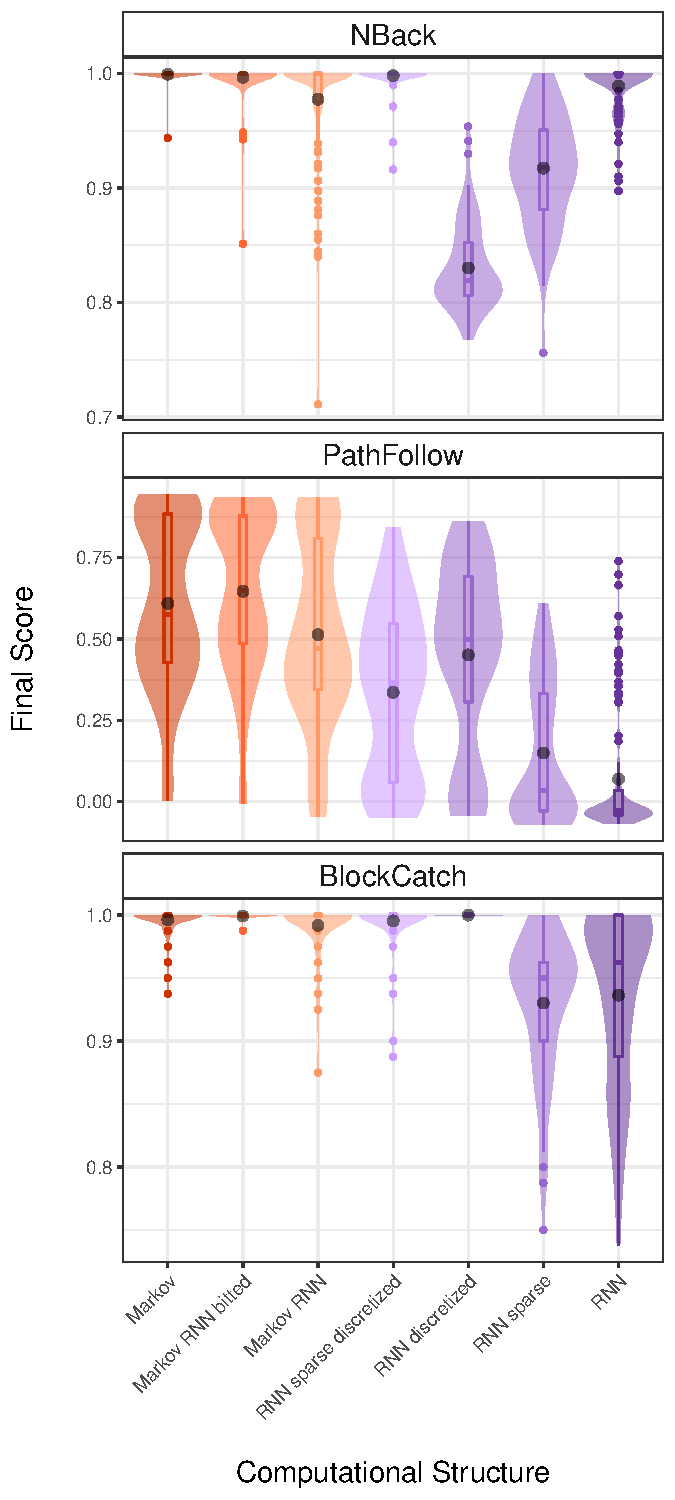
\includegraphics[width=0.45\textwidth]{chapters/2-comp-hybrid/figs/merged_LOD_data_end_score.pdf}
    \caption{Performance of computational structures across tasks. Color hue indicates the brain variant used; color saturation indicates distance in number of changes from canonical structures, with more distant hybrids being less saturated. Note the varied scales on the y-axis, as we are interested here only in comparative performance within worlds rather than across worlds.}
    \label{fig:scores}
\end{figure}

\begin{table}
\input{chapters/2-comp-hybrid/tables/nback}
\bigskip
\input{chapters/2-comp-hybrid/tables/pf}
\bigskip
\input{chapters/2-comp-hybrid/tables/blockcatch}
\bigskip 
\caption{Differences (p-value) between mean performance on tasks (A) NBack, (B) PathFollow, and (C) BlockCatch. Green cells indicate significant difference. P-values corrected using Tukey method for a family of 7 estimates. * $= p \leq 0.05$; ** $=p \leq 0.01$; *** $=p \leq 0.001$. }
\end{table}

We present here results from an application of the Comparative Hybrid Approach where we compare Markov Brains and RNNs as a demonstration of the method's qualitative analytical power. 
By identifying architectural differences between brain types and creating intermediate ``hybrids" of the two computational structures, we gain the ability to analyze how performance varied across hybrid structure and task. 
We are then able to examine whether our assumptions about the architectural differences separating the substrates map to the quantitative difference separating their performance.

\subsection{Primary Results Analysis}

We saw that Markov brains generally suffered significant performance loss when their logic lookup table gates were replaced with RNN-like threshold gates with continuous values. 
However, performance was stable or even increased when those threshold gates were used in consort with discrete memory. 
This indicates that discretization, rather than the logic lookup table structure, accounts, at least in part, for the high performance of Markov Brains on the tasks we investigated. 
The results are not as clear when we consider the RNN variants. 
While we can clearly see that the RNN variant which is both sparse \textit{and} discretized out perform canonical RNNs in all three tasks, changes in independent task performance do not clearly indicate whether it is sparsity or discretization that is the primary factor---in fact, the results indicate that the benefits conferred by each feature are task dependent.

Overall, from these results, we tentatively conclude that discretizing outputs results in generally higher performance than biasing towards network sparsity. 
However, we note that all versions of Markov Brains tend to have higher sparsity compared to all versions of RNN, and so we can not discount that sparsity plays a significant role in explaining Markov Brains' generally higher performance.

\subsection{Cross-Brain Examination: Discretization}

\subsubsection{Discretization Helps Performance on BlockCatch and PathFollow} In two of the tasks, BlockCatch and PathFollow,  discretizing the RNN memory resulted in significant performance gains, while sparsity of the network had little effect. 
In addition, the effect of combining sparsity and discretization resulted in performance that was lower than that of the RNNs that were only discretized.
In all cases, hybrid Markov Brains (i.e. with RNN gates) display higher performance when discretized (i.e. bitted) in these same tasks. 
Moreover, we were surprised to see that in PathFollow, the Markov ANN bitted hybrids outperform the canonical Markov Brains.

\subsubsection{Discretization or Sparsity Alone Hinder, But Together Help in RNN Hybrids Performance on NBack} The advantages of discretization do not carry across all types of tasks as the results from NBack attest. 
The RNN NBack results are clearly different than the other two tasks in multiple ways; we see a performance gain \textit{only} in the combined sparse-discretized network where as discretized-only and sparse-only RNN hybrids experienced performance \textit{loss}.

\subsection{Other Factors To Consider}
Based on the contradictory results observed in relation to the NBack task, we turn to the examination of other specific brain features and task details for insights that might help to explain these results. 
The following are some conjectures on possible explanations for our observed results, and should be seen as theoretical.

\subsubsection{Potential Influence of Encoding} It is possible that only considering the difference between the RNN and Markov Brain architectures is insufficient to explain the differences in performance.  
Even though both structures are built from the same type of genomes with the same mutational properties, the process which is used to map the genomes to the two types of brains is quite different. 
RNNs use a direct encoding method where a contiguous region at the beginning of the genome is read and each position in the genome relates to a particular feature in the brain (a bias or a weight). 
In contrast, Markov Brains rely on biologically inspired ``start codons" that mark coding regions. 
The RNN encoding means that the number of coding sites in the genome is constant, but because the number of start codons in a Markov Brains genome can vary, the number of coding sites can also vary. 
This results in a fixed number of effective mutations in RNNs but a variable number of effective mutations in Markov Brains. 
Because of these differences in encoding, the ways that brains are affected by mutation and the resulting evolutionary pathways may be very different. 
Further consideration of this is outside of the scope of this work, but we stress that the encoding methods could account for differences in observed performance and that future work should consider comparisons of encoding methods.

\subsection{Information Integration}

One factor that we believe could be critical to understanding these results and the results of our proposed method in general relate to the cognitive and memory requirements of the tasks being used. 
In two of the tasks, BlockCatch and PathFollow, we saw a gradient of performance across hybrids as we generally expected. 
The alterations of the RNNs caused them to perform more similarly to the Markov Brains (high performance), and the alterations of the Markov Brains caused them to perform more similarly to the RNNs (lower performance). 
However, this was not the case in the NBack task.

If we consider all three tasks from the standpoint of the cognitive abilities that each task requires, we can see that NBack only requires simple feed forward memory, while the other two tasks require long term memory and some level of information integration. 
Information integration is the ability to arrive at an answer that requires more than simple memory. 

NBack can be solved by an agent that simply stores the incoming bit string in a ``delay" buffer and delivers these stored values to the correct outputs over time. 
Each output relies only on a single prior input.

In PathFollow, agents must be able to integrate information over time. 
When the agent starts on a new path, they do not yet know which turn signal is associated with which turn. 
They must use trial and error to establish if they are in a ``$0$ means left and $1$ means right" path or a ``$1$ means left and $0$ means right" path. 
This requires that they make a guess when they arrive at the first turn signal. 
If they stay on the path then they ``know" that they guessed correctly, but if they step off the path then they must not only remember that they guessed incorrectly, but also must navigate back onto the path. 
During this process (of getting back onto the path) their sensors will not provide them with any useful input, so they must remember what part of the path recovery process they are executing. 
Finally, integration over sensors is needed. 
In order to detect a turn signal, agents must look at at least two inputs: the ``turn signal" input, and either the ``on turn" input or both the ``on forward" and ``off path inputs".

Finally, Block Catch requires that agents identify the size and direction of falling blocks. 
The identification of the left/right direction requires information integration (i.e. at least the integration of sensor states from consecutive time steps), while the identification of block size can be achieved by integration over time and sensor space or just over time.

From this it follows that the optimal logic and wiring for NBack should be simple and sparse. 
In fact there is no advantage in NBack to being able to integrate or even alter the input values. 
Arguably, a ``pass though" gate which simply moves a single value from T to T+1 should be optimal. 
It is unclear why canonical RNNs perform well on NBack versus the discretized-only and sparse-only hybrids but we conjecture that these intermediate hybrids resulted in less navigable fitness landscapes. 
 
PathFollow and Block Catch both require more complex models of memory and more complex methods of manipulating data than NBack. 
We believe that this accounts for the primary variance between the results of NBack and the results of PathFollow and Block Catch.

While this study was not designed to detect how information integration may impact optimal cognitive structures, our results indicate that such integration should be considered in future work.

\section{Conclusion}
% FINAL?

We present these results as an illustrative example of the Comparative Hybrid Method and how it can be applied to analyze key components of digital brain architectures. 
By creating hybrids of existing examples of neuro architectures, we are able to test computational structures in a piece wise manner on a collection of tasks of varying complexity. 
The comparative performance of the unmodified and hybrid brains can be used to make inferences about how computational components and structure may relate to task success and ultimately to understanding fundamentally why the unmodified brains behave differently.

In practice, this technique can be extended to any two or more structures whose performance you are interested in comparing.
All that is required is an intuition for what architectural differences separate the two computational structures, and an implementation of hybridized versions altering each of those components in turn. 
While such a task may be in some cases practically unwieldy, it will in many cases be simpler than the alternative of analytically examining the entire brain architecture at once and altering all possible parameters in order to identify key components.

In theory, the effects of the comparative hybrid model could extend into biological systems. 
As the ability to accurately simulate neuron models progresses, our method could be used across a continuum of neuron models and with the right advances in bio-engineering, the biological brain itself. 
Ultimately we believe that the Comparative Hybrid Method will allow us to single out key variables of cognition that could provide a path to a better understanding of intelligence, whether it be biological or computational. 
\section{Acknowledgements}% FINAL

This material is based in part upon work supported by a National Science Foundation Graduate Research Fellowship to A.A. and by the National Science Foundation under Cooperative Agreement No. DBI-0939454. 
Any opinions, findings, and conclusions or recommendations expressed in this material are those of the author(s) and do not necessarily reflect the views of the National Science Foundation. 
Michigan State University provided computational resources through the Institute for Cyber-Enabled Research. 
Michigan State University occupies the ancestral, traditional, and contemporary Lands of the Anishinaabeg–Three Fires Confederacy of Ojibwe, Odawa, and Potawatomi peoples. 
The University resides on Land ceded in the 1819 Treaty of Saginaw.
\section{Author Contributions}% FINAL

C.B.~conceived of the presented idea and study design. 
S.A.~provided empirical backing for the theoretical design. 
C.B.~developed components of the code base for the project. 
A.A.~and C.B.~performed computation and data collection. 
S.A., A.A., and C.B.~performed data analysis and interpretation. 
S.A.~drafted the initial manuscript. 
C.O. provided significant guidance on the manuscript. 
S.A., A.A., C.O., and C.B.~revised and approved of the final manuscript. 

\chapter{Tessevolve: An interface for visualizing evolutionary fitness landscapes in 4D}
\label{ch:vr-viz}

\noindent Authors: Acacia L. Ackles and Emily Dolson\\
This chapter is adapted from an upcoming publication in revision to be submitted to IEEE VIS 2023.

% some great advice from betty cheng
% https://www.cse.msu.edu/~chengb/Writing/intro-guidelines-stirewalt.txt
\section{Introduction}

Evolution, once firmly in the domain of biologists, is now understood to be a fundamental algorithmic process with wide applicability across fields. 
Computer scientists and engineers in particular have recently made many advances towards understanding and harnessing evolution. 
Evolutionary dynamics have been applied, for example, to develop self-driving cars \citep{abuzekry_comparative_2019}, design radio antennae for satellites \citep{oreilly_evolved_2005} , and advance the state of the art for machine learning \citep{vikhar_evolutionary_2016}. 

% Depending on space, we could potentially hammer a little more on the recent successes of evolutionary computation here

Across these various domains, experts are frequently interested in understanding not only how evolution has proceeded in the past, but where it might continue in the future. 
Such insights facilitate better understanding of the capabilities and limitations of their evolving system of interest. 
In these cases, experts are interested in understanding the search space of their particular problem and how evolution traverses that space (hereafter called ``evolutionary space"). 
Strong intuition for the topological properties of a given search space promote accurate inferences and predictions about how evolution will proceed in that space.

%As in all data analysis tasks, data visualization is a powerful tool for gaining such intuition.
%Good data visualizations are a particularly powerful way to build such intuition, as they do not need to rely on mathematical or domain-specific knowledge and can be broadly applicable across fields. 

To facilitate this intuition, search spaces are often represented as fitness landscapes.
In these representations of evolutionary space, high-fitness areas of the search space are represented as peaks and low-fitness areas are represented as valleys. 
This visual metaphor is ubiquitous and powerful, and its usefulness lies in its familiarity; it draws upon topographical representations which most people will have encountered in multiple other contexts. 
However, this familiarity can be misleading as it encourages us to think about landscapes in terms of only three spatial dimensions, whereas true evolutionary landscapes can have vastly more dimensions. 

Indeed, mathematical work suggests that the fitness landscape metaphor has mislead evolution researchers. 
High-dimensional fitness landscapes may have qualitatively different properties that lead evolution to behave very differently than it would in a low dimensional landscape \citep{agarwala_adaptive_2019}. 
This problem has lurked in the background of evolutionary theory research for over a decade \citep{kaplan_end_2008}. 
It is frequently stated as a caveat, but low-dimensional fitness landscapes continue to be used routinely for their immense intuition-building power.

Building intuitions with a data visualization known to potentially produce misleading intuitions is not ideal. 
To begin remedying this problem, we developed \textit{Tessevolve}, a web-enabled virtual reality (VR) based tool for visualizing fitness landscapes in 2D, 3D, and 4D. 
This platform enables users to begin building intuition for how fitness landscapes change as they gain dimensions. 
Additionally, it allows them to plot evolutionary data on top of the fitness landscape, to understand how the higher numbers of dimensions affect evolutionary dynamics. 
While four dimensions is still far fewer than most real world fitness landscapes contain, the ability to compare three dimensional landscapes to four dimensional landscapes enables a substantial advance in our ability to comprehend the effects of adding dimensions.

To our knowledge, Tessevolve is the first 4D visual representation of the evolution of a lineage and its surrounding landscape. 
Furthermore, for both 3D and 4D landscapes, domain experts found Tessevolve more intuitive and easier to use than existing visualization methods. 
Here we present the development and use cases for Tessevolve in detail, and highlight some of the insights made possible with this novel visual interface.
\section{Domain Background}
A central goal in evolutionary research is to understand the trajectory evolution took in the past and predict the trajectories it is likely to take in the future. 
Both the reconstruction of the past and prediction of the future require a strong working model of the evolutionary search space; that is, what combinations of traits might an organism have, and how do those combinations lead to reproductive success or failure? 
Consider as a simplifeid example the fitness of a tree; two traits of interest might be the depth and breadth of its root system.
One might be able to quantify the fitness impacts of these two traits and write an optimization function to find the maximum. 
Finding the maximum fitness, however, is of limited use when you don't know if evolution can actually find the necessary combination of traits; an extremely deep and extremely wide root system might be helpful, but also energetically infeasible.
Thus, it is frequently much more important to understand the trajectory that evolution will take through the problem space.
Such knowledge is particularly critical for efforts to prevent the evolution of dangerous traits (\textit{e.g.} antibiotic resistant bacteria) by precisely controlling the trajectory of evolution \citep{iram_controlling_2021}.
It is therefore useful to have some way to visualize the entire domain of the traits of interest as they relate to fitness.

\begin{figure}
    \centering
    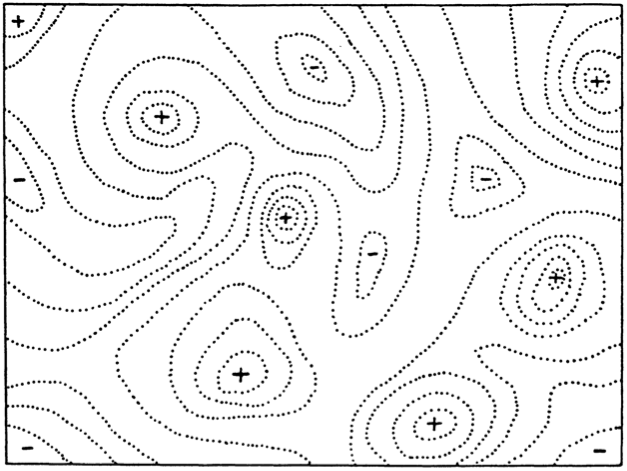
\includegraphics[width=0.5\textwidth]{chapters/3-vr-viz/figs/wright.png}
    \caption{Original fitness landscape schematic from Wright (1932). Plus signs represent peaks while minus signs represent valleys. Dotted lines indicate changes in altitude (that is, changes in fitness).}
    \label{fig:bkg:wright}
\end{figure}

\subsection{Evolutionary Fitness Landscapes}
The current predominant method of visualizing the evolutionary search space is the \textit{evolutionary fitness landscape}. 
This visual metaphor, created by Sewall Wright \citep{wright_roles_1932}, depicts two traits as $x$ and $y$ coordinates with fitness as a third $z$ coordinate, often represented as height (\autoref{fig:bkg:wright}). 
The result is indeed a landscape-like appearance, which brings a sense of intuitive familiarity to the reader; higher fitness areas are easy to spot, and movement around the space is easy to imagine. 

Such a familiar depiction has made fitness landscapes a nearly ubiquitous visual metaphor. 
Evolution research across fields frequently uses the terms ``peaks" and ``valleys" to describe areas of high and low fitness respectively. 
Furthermore, populations moving from low-fitness regions to high-fitness regions are said to be ``hill-climbing", while populations moving through low-fitness regions are ``valley-crossing". 
These terms and the image of the underlying landscape are descriptive and easily understandable; unfortunately, they can also be severely misleading as to the true nature of evolutionary space.

\subsection{Loss of Information \& Intuition}

One obvious shortcoming of the topographical fitness landscape is that it depicts only two traits and therefore encourages imagination of the evolutionary space in only three dimensions. 
However, most real-world evolutionary spaces are extremely high-dimensional; any trait an organism possesses might be considered a dimension of the evolutionary landscape. 
Some conceptualizations go even farther, treating the identity of the nucleotide at each position in an organism's DNA sequence as a separate dimension. 
Intuition about movement across low-dimensional spaces does not always translate well to intuition about similar movement across high-dimensional spaces \citep{agarwala_adaptive_2019}; therefore, relying on 2D visual landscape metaphors can mislead us about certain evolutionary dynamics.

One such evolutionary dynamic of particular interest is the aforementioned \textit{valley-crossing} problem. In the fitness landscape metaphor, both local and global maxima are represented as peaks. At one of these peaks, any small mutation of a trait will necessarily shift the population to an area of lower fitness, and evolutionary pressure will then return the population to the peak. How then are populations able to move from local maxima to global maxima when they are effectively buffeted away from moving through the intervening areas of low fitness?

Research inspired by intuitions from low-dimensional landscapes tends to approach this problem with the implicit assumption that valley crossing requires 1) multiple mutations to occur at once, or 2) a sequence of individuals with deleterious (\textit{i.e.} fitness-reducing) mutations to survive long enough to have an offspring that lands on the opposite side of the valley. Much effort has been devoted to understanding what conditions allow these scenarios. However, researchers skilled in understanding the mathematical properties of high-dimensional landscapes have suggested that this is the wrong question \citep{kaplan_end_2008, gavrilets_2010}. In high dimensional spaces, they argue, the probability of a valley existing in all dimensions simultaneously is very low. In this view, populations do not need to cross valleys and instead likely drift across neutral ``ridges'' between the peaks. This phenomenon is sometimes referred to as an ``extradimensional bypass'' -- a path along one dimension that connects two peaks \citep{cariani_extradimensional_2002}. %Another approach 

%There are multiple good explanations of how populations undergo or avoid valley-crossing, such as imagining landscapes as ``holey" binary surfaces rather than topographies, or identifying multiple mutations which could ``launch" organisms from peak to peak across valleys. However, one simple explanation is that our intuitive, fitness landscape based idea of ``fitness valleys" is itself problematic; in high-dimensional spaces, ``peaks" may be so frequent and so close together in evolutionary space that valley crossing presents no problem if mutations are of any appreciable size (CITE). 

In this case, it would seem that attempts to visualize fitness landscapes as three-dimensional surfaces are not aiding scientific discovery and are in fact hindering our understanding. This issue has been well-known for over a decade and is severe enough that some domain experts have called for an end to the fitness landscape metaphor altogether \citep{kaplan_end_2008}, but the metaphor remains popular. Many people think most clearly about problems when they have a thorough mental image of them. Asking them to abandon that mental image without providing a better replacement is not an ideal solution. Thus, we suggest that the most beneficial next step for the community is to build an improved intuition for the ways in which low-dimensional fitness landscape visualizations may mislead us. If the fitness landscape metaphor is to continue being used, evolutionary scientists need a visceral understanding of where it is useful and where it falls short. Here, we seek to do exactly that. 

\subsection{Holey fitness landscapes}

Another influential way of thinking about high-dimensional fitness landscapes, is the idea of holey fitness landscapes \citep{gavrilets_evolution_1997}. This concept is inspired by the idea that, in realistic fitness landscapes, nearly all high-fitness genotypes are mutationally adjacent to other genotypes of comparable fitness. Thus, it may be useful to abstract a high dimensional landscape by compressing the space of possible fitnesses to two: viable and not viable. The resulting search space can be visualized as a plateau (the viable genotypes) with holes cut out of it (the not viable genotypes). Evolution in such a space is a matter of neutral diffusion along the plateau, and can be modeled as a percolation process \citep{gavrilets_high-dimensional_2010}.

While this model has been criticized both for abstracting away important dynamics and for being misleading in its own way \citep{kaplan_end_2008}, it has so strongly influenced thinking on how best to conceptualize high-dimensional fitness landscapes that we would feel remiss in not mentioning it here. Although we have yet to explicitly incorporate this thinking into Tessevolve, it suggests a variety of valuable future directions.
\section{Related Work}

There is clearly demand for a multidimensional alternative to the fitness landscape metaphor which can help develop the intuition for evolutionary space provided by such a simple visualization. Multiple approaches to this multidimensional problem currently exist; however, they suffer from problems with scaling  and in some cases fail to provide intuition about the movement of lineages across the space over evolutionary time.

Here we present the current standard in fitness landscape visualization in more than two dimensions, as well as inspirations for our own extension into 3D and 4D landscape-based visualizations in virtual reality. 

\subsection{Graph-Based Visualizations}

The current standard for visualizations beyond two dimensions is to present a graph-based model. 
The most typical representation, which we term network models, is to represent the search space as sparsely connected network.
An alternative model termed Hyper-Space Graph Paper instead represents the space as a grid of systematically arranged trait combinations.

\subsubsection{Network Models}

\begin{figure}
    \centering
    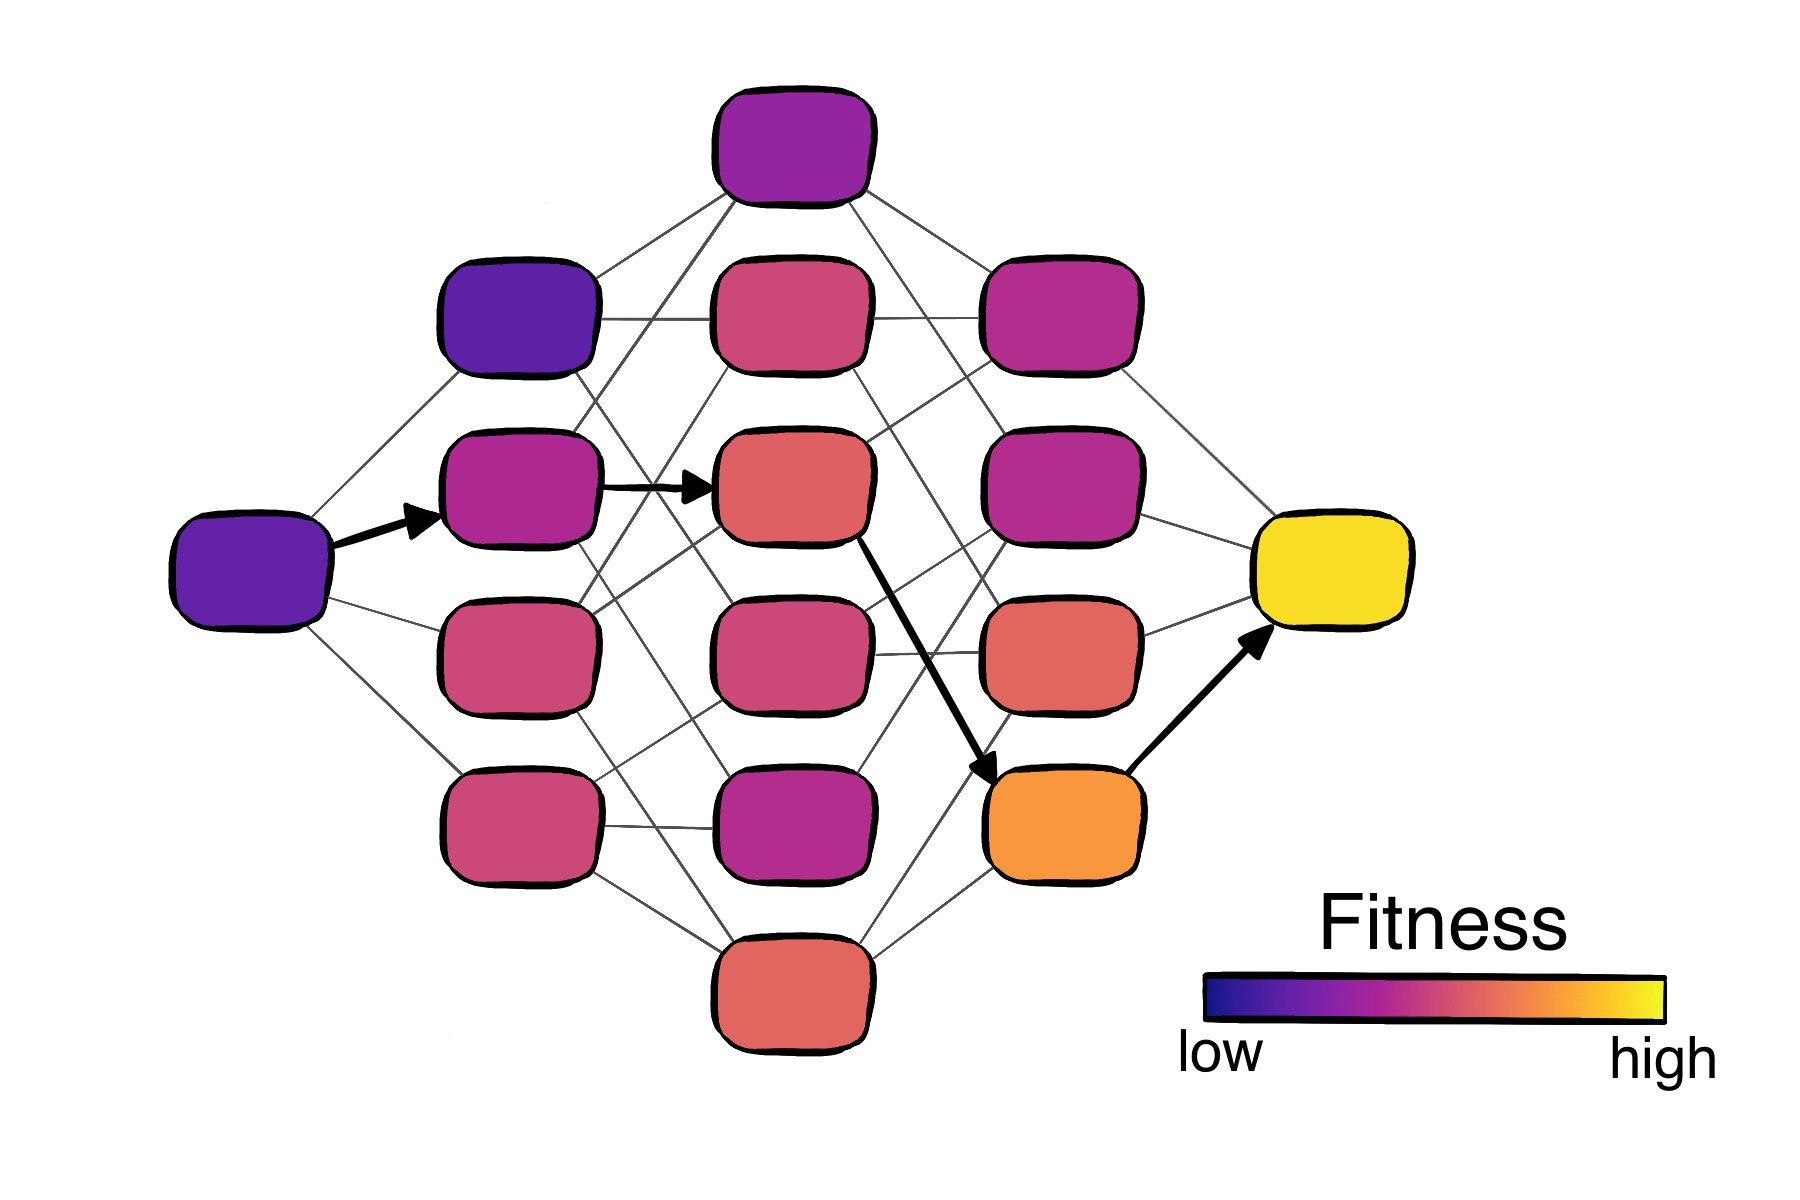
\includegraphics[width=0.5\textwidth]{chapters/3-vr-viz/figs/network.png}
    \caption{Network model of a fitness landscape. Lines indicate genotypes which are adjacent in evolutionary space. Colors indicate fitness according to key. Arrows denote traversal of the landscape. Adapted from Wu et al., 2016. Image by Katie Gleason.}
    \label{fig:related-work:network}
\end{figure}

Network models are perhaps the most popular way to represent higher dimensional evolutionary search spaces.
In these models, nodes represent genotypes while edges represent proximity; connected nodes are adjacent genotypes. \citep{mccandlish_visualizing_2011}.
Directed edges in these visualizations can represent either the observed behavior of a lineage traversing the space, or the direction of increasing fitness.
Lineage trajectories are also sometimes represented by the color of edges and node outlines \citep{ogbunugafor_competition_2017}.
Fitness can be represented visually in a multitude of ways: as labels on the nodes \citep{ogbunugafor_competition_2017}, node size \citep{mccandlish_visualizing_2011, iram_controlling_2021}, or colorings of the network \citep{wu_adaptation_2016, jimenez_comprehensive_2013}. 
An example of a network model with fitness mapped to node colorings is provided in \autoref{fig:related-work:network}.

A common use of network models is to represent landscapes composed of presence/absence data for a small number of genes (often four). In evolutionary medicine, a number of empirically-derived landscapes of this form exist \citep{mira_rational_2015, ogbunugafor_adaptive_2016}. With four genes to consider, there are 16 possible genotypes. These 16 genotypes can be arranged in an intuitive pattern where all mutationally-adjacent genotypes are adjacent to each other. Such a landscape is four dimensional (indeed, these visualizations are sometimes referred to as tesseracts). However, this intuitive visual representation is only possible because each of the dimensions is constrained to the values zero and one. %Intuitive graph layouts are more challenging for five dimensions, and have yet to be discovered for higher number of dimensions.

Overall, network models do not suffer the information loss problem of 2D and 3D topological representations; every candidate genotype is represented as a node in the network. 
Proximity in evolutionary space is also intuitive, represented by edges connecting nodes. 
However, intuition is limited by the size of the network, which is determined by the number of traits as well as the number of values each trait can take on.
For very large networks, visualization quickly becomes messy as the number of edges grows rapidly.  
Additionally, dynamics of interest such as ruggedness valley crossing are difficult to visualize; however, see \citep{ogbunugafor_competition_2017} for one visual option.
Finally, a particularly difficult limit of network models is that they are by necessity discrete; continuous-valued landscapes or lineages cannot be visualized with a finite number of nodes.

\subsubsection{Hypergraphs}

Hyperspace Graph Paper (HSGP) is an alternative graph-based model that takes advantage of recursive structure to aid in intuition. 
HSGP represents binary strings of length $n$ as the corners of an $n$-dimensional hypercube, then ``unfolds" that cube to produce a flat grid representation \citep{wiles_hyperspace_2006}. 
Adjacent genotypes have self-similar placement within sub-grids, and fitness is represented via shading (\autoref{fig:related-work:hgsp}). 

\begin{figure}
    \centering
    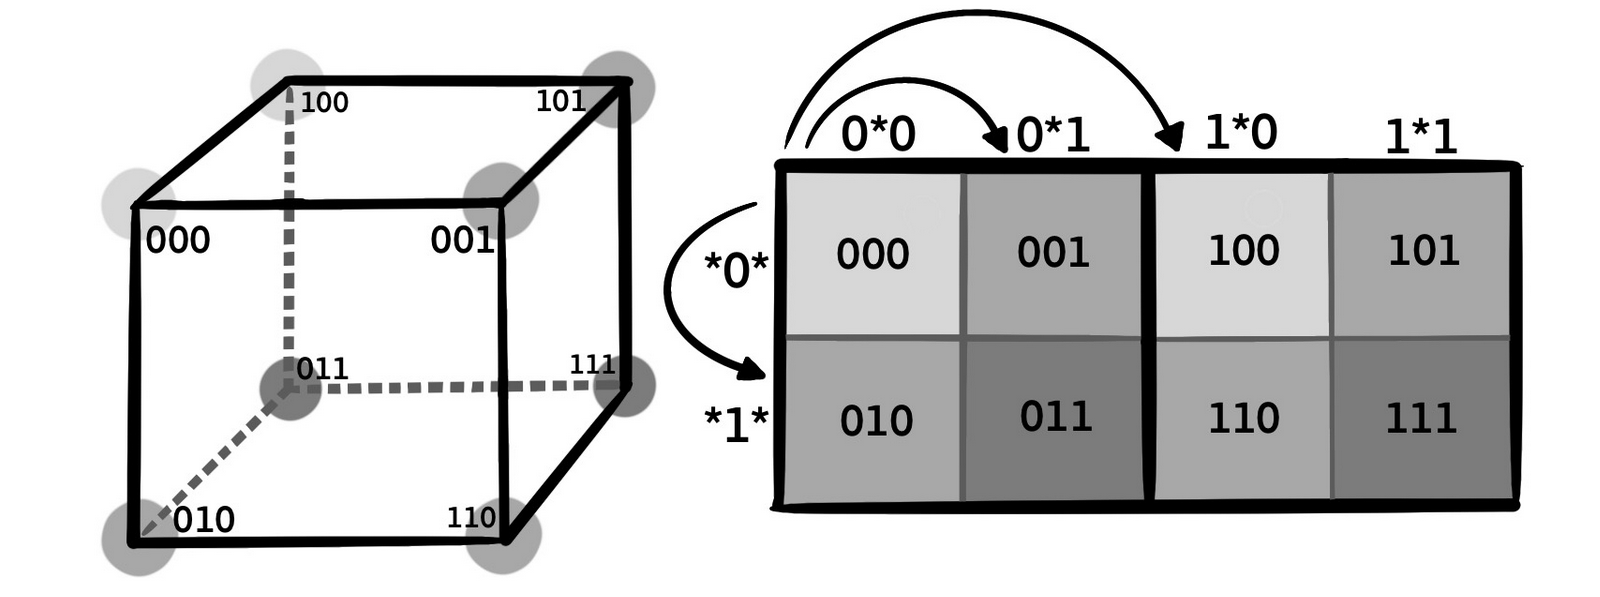
\includegraphics[width=0.5\textwidth]{chapters/3-vr-viz/figs/hsgp.png}
    \caption{Hyperspace graph paper example in 3D. Each corner of the cube is ``unfolded" to create a flat grid structure. Arrows are for demonstration purposes to indicate how adjacent corners in the cube are positioned in the unfolded grid. Greyscale represents fitness, where more saturated greys are higher fitness. Adapted from Wiles et al., 2003. Image by Katie Gleason.}
    \label{fig:related-work:hgsp}
\end{figure}

One advantage of HSGP visualizations, as in the network models, is that they are lossless; each point in fitness space directly translates to a position in the grid, so no information is discarded. 
Unlike network models, edges are not explicitly drawn, reducing the visual noise for larger landscapes. 
For HSGP models it is possible to view global and local maxima at a glance, even in problems with multiple optima \citep{wiles_mapping_2003}. 
However, they still share one of the major shortcomings of network models: they are limited to discrete landscapes, and in particular to landscapes which can be binary-coded. 
Additionally, since adjacency in evolutionary space does not map directly to adjacency in the visualization, viewing lineage traversals across the landscape is messy and unintuitive. 

Network-based models do not suffer from the same dimensionality loss as landscape-based models, but this ability to expand to multiple dimensions does not necessarily mean those expansions are intuitive.
Many of the limitations of network-based models are due to either attempting to combine a lot of information into limited spatial dimensions (i.e.~a 2D image) or due to their lack of spatial structure (i.e.~poor representation of proximity in genotype space vs.~fitness space). 
Therefore, we turn to more spatially-based models to build intuition for higher dimensions.

\subsection{VR-Enabled Visualizations}

Virtual reality is increasingly used to push the boundaries of data visualization. Previous studies have shown the use of VR can support better intuition for spatial data \citep{ambinder_human_2009}, provide a faster overview for big data visualizations \citep{olshannikova_visualizing_2015}, and provide deeper insight into the true structure of imaging-related data \citep{el_beheiry_virtual_2019}. However, the use of VR to study evolutionary data generally, and fitness landscapes specifically, has been extremely limited.

\subsubsection{2D Landscapes in VR}

\begin{figure}
    \centering
    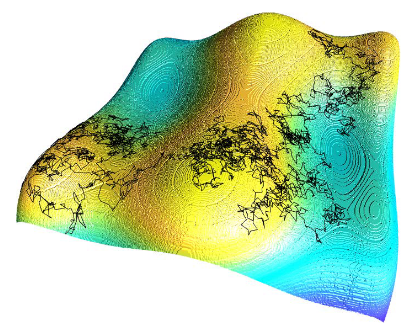
\includegraphics[width=0.5\textwidth]{chapters/3-vr-viz/figs/2dviz.png}
    \caption{2D landscape visualized in virtual reality. Black line represents a lineage traversing the landscape.}
    \label{fig:related-work:2dviz}
\end{figure}

There is no prior work on using VR to visualize higher-dimensional landscapes, but VR has been used to visualize 2D fitness landscapes \citep{dolson_visualizing_2018, dolson_interpreting_2020}. 
Here, as in the topological representation, the genotype is represented as a point on the cartesian plane. 
The spatial capabilities of VR are leveraged to show fitness as height, analogous to a 3D relief map (\autoref{fig:related-work:2dviz}. 
This use of VR avoids the problems inherent to projecting 3D graphs onto 2D pages or planes. 

The ability to visualize landscapes in their full spatial context allows for greater insight into evolutionary dynamics across the landscape; for example, lineages can be traced ``through" peaks rather than ``over" them \citep{dolson_visualizing_2018}. 
However, this visualization is still limited to 2D landscapes and therefore is subject to many of the same issues as the topographical projection, albeit with improved interpretibility and visibility. 

\subsubsection{Breaking into the Fourth Dimension}

It is relatively simple to imagine how one might represent a 3-dimensional landscape in a 3-dimensional space, but it is more difficult to imagine representations for a 4-dimensional landscape. 
The fourth dimension essentially must be projected into the 3-dimensional space, casting a 3-dimensional ``shadow". 
The viewer can then see slices of the fourth dimension by viewing 3D space. 
However, these slices cannot be viewed concurrently, so we require a way to step through successive slices. 

One option is to display 3D slices in a grid format, as in one medical application termed ``Bento Box" \citep{johnson_bento_2019}. 
This approach allows users to simultaneously view multiple slices, which can be helpful for comparative analysis. 
However, since this approach requires rendering all slices to the screen at once, it is computationally costly for the graphical software.

Another approach is to allow the viewer to scroll through three-dimensional slices, analogous to an MRI scan. 
Slices of a fourth-dimensional object are displayed one at a time, with the viewer able to scroll through the slices at will.
This allows for smoother rendering and user control, while sacrificing the comprehensive view from the Bento Box approach. 

Using a combination of inspiration from 2D fitness landscapes in VR and existing techniques to visualize 4D landscapes, we can identify key components to visualize 3- and 4-Dimensional fitness landscapes in virtual reality. 
\section{Domain Requirements and System Overview}

Based on the above literature, conversations with domain experts, and our own experience as active researchers in the field, we identified five key requirements for a new VR-based fitness landscape visualization and incorporated them into our final design.

\subsection{Requirements}

The following requirements were identified as essential to the design to meet the goal of gaining spatial insight into how fitness landscapes behave across dimensions.

\paragraph{\textbf{R1: Spatial Insight.}} Experts must get a sense of depth, distance, and scale within a three-dimensional space in order to build spatial intuition.

\paragraph{\textbf{R2: Ease of Access.}} Experts must have access to the visualization even without virtual reality hardware in order to increase reach and usability.

\paragraph{\textbf{R3: Ease of Interpretation.}} Experts must be able to interpret the visualization without drawing upon mathematical background knowledge.

\subsection{System Overview}

Tessevolve (\textbf{tess}eract $+$ e\textbf{volve}) is a web-enabled three dimensional fitness landscape visualization built to address the domain requirements listed above. With this visualization, we seek to expand intuitive understanding of crucial domain concepts such as landscape ruggedness and lineage traversal. We address R1 (Spatial Insight) by implementing the visualization in an established virtual reality framework which handles depth and distance. This framework is hooked into a web-enabled interface so as to be accessible through any internet connected device to address R2 (Ease of Access). Finally, we solicit and report qualitative feedback from experts on the intuitiveness of design to address R3 (Ease of Interpretation). 
\section{Implementation of Tessevolve}

Here we describe in depth the data model, design choices, and implementation features involved in the development of Tessevolve. Our visualization makes use of 3D projections in virtual reality to scale up the fitness landscape metaphor into multiple dimensions. We use the emerging digital evolution platform MABE2 to generate evolutionary data, the ALife Data Standards Python package to process lineage information, and the open-source platforms A-Frame, D3.js, and Bootstrap to create easily accessible web and VR interfaces for the final data visualization. The result is a fully open source visualization of complex, multidimensional phylogenetic and evolutionary data. The full GitHub repository for the project, including all scripts involved in data generation, pre-processing, and visualization, is available at \url{https://github.com/alackles/tessevolve} \citep{ackles_alacklestessevolve_2022}, and the platform itself is accessible at \url{https://alackles.github.io/tessevolve}. Note that for all figures in this paper, due to the nature of the images, they would likely better be viewed at the live demo linked above.
% change github URL to DOI before submission

\subsection{Data Model}

Currently, there is no broadly accepted standard for fitness landscape data. Our data model therefore accepts data in CSV format, with initial columns \texttt{x0, x1, x2, x3} representing the traits of interest, and a column \texttt{fitness} which represents the fitness associated with those trait values. Columns \texttt{x2} and \texttt{x3} are optional dependent on the dimensionality of the underlying landscape (i.e., a 3D landscape would only have columns \texttt{x0, x1, x2, fitness}). 

We were also interested in visualizing lineages' evolution (phylogenetic data) across these fitness landscapes. Since in this case the data we visualized was from computationally evolved organisms, we use the ALife Data Standard for phylogenetic data \citep{lalejini_data_2019}. In this standard, information about an organisms's traits is recorded every time a new lineage forms. In the future, Tessevolve could be expanded to accept phylogenetic data in other formats such as the biologically-standard Newick format.

\subsection{Data Generation and Pre-Processing}

To generate the fitness landscapes used for our web demo of Tessevolve, we turned to the CEC'2013 Benchmark functions which provide both Python and C++ (among other languages) implementations of multiple functions across dimensions \citep{li_benchmark_2013}. The fitness landscape data itself was generated using the Python implementations, while the C++ implementations were incorporated into the digital evolution platform MABE2 (https://github.com/mercere99/MABE2) to generate lineage data. We then used the ALife Standards Python package to process the lineage data into a standardized CSV format for the visual front-end \citep{lalejini_data_2019}.

% I have no idea if we need to add more information here. 

\subsection{Virtual Reality Engine}

Virtual reality allows for users to take maximal ability of the brain's ability to build intuition about physical spaces. By being immersed in the visualization, they can develop a visceral understanding of how it behaves. However, to promote accessibility, it is ideal for VR visualizations to also be viewable in a web browser, as a fallback. By allowing web users to manipulate the visualization with their mouse, such a format can still provide a far better experience than a static 2D projection.

To this end, we chose to implement Tessevolve using the webXR specification, which supports browser-based VR scenes that can be viewed in a browser in addition to on a VR headset. Specifically, we used Mozilla's AFrame framework \citep{mozilla_-frame_2022}, which facilitates building a VR visualization out of html components. This structure allows it to play nicely with d3.js \citep{bostock_d_2011}, which we used to connect the data into the visualization.

\subsection{Design Choices}

The most crucial design decision we had to make was how to display the 3D landscape in a way that was both intuitive and informative. In particular, we needed to decide how users would be able to see multiple points in a landscape simultaneously. For example, a true 3D analogue to the traditional 2D landscape would be akin to an aquarium tank, where every spot in the 3D space conveys some visual information about the fitness at that point. However, such a design would completely block the vision of the viewer when they are inside the landscape; there is no space to see ``around" any component to investigate other regions (\autoref{fig:imp:spheres}) 

\begin{figure}
    \centering
    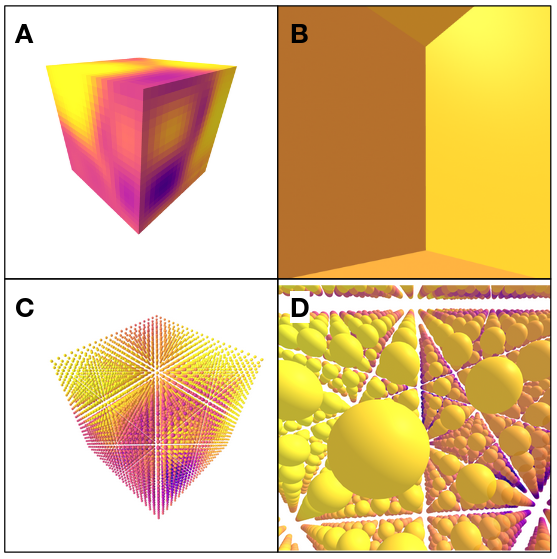
\includegraphics[width=0.5\textwidth]{chapters/3-vr-viz/figs/spheres.png}
    \caption{Illustration of the challenges of having a continuous 3D landscape visualization. (A) A landscape visualization where all genotypes are displayed. (B) The poor view from inside \textit{A}. (C) A landscape visualization where genotypes are displayed at fixed, discrete intervals. (D) The view from inside \textit{C}.}
    \label{fig:imp:spheres}
\end{figure}

We therefore chose to display discrete, evenly-spaced points on the landscape rather than a continuous mesh. These points are displayed as spheres at 90\% opacity, allowing for both distant and nearby inspection of the landscape. While this technique somewhat reduces the resolution of the fitness landscape, it greatly increases its interpretability. 

Another challenge was how to indicate the fitness at each point when all three of our spatial dimensions are used to convey information about trait values. For this purpose, we use a color scale, as is commonly implemented to visualize imaginary functions. This method should be easily recognizable to domain experts due to its frequent use in other mathematical visualizations. We chose to use the viridis color scheme plasma variant as it is both colorblind friendly and maps ``cool" colors to low values and ``warm" colors to high values, further increasing familiarity.

We also wanted to display lineage data on landscapes. We represent newly born taxa as cubes to distinguish from the landscape's spheres, and consecutive taxa are connected by a simple line. The color scheme for the fitness of each taxon is the same as that of the landscape. 

\subsection{Visualization Interface}


\begin{figure*}
    \centering
    \fbox{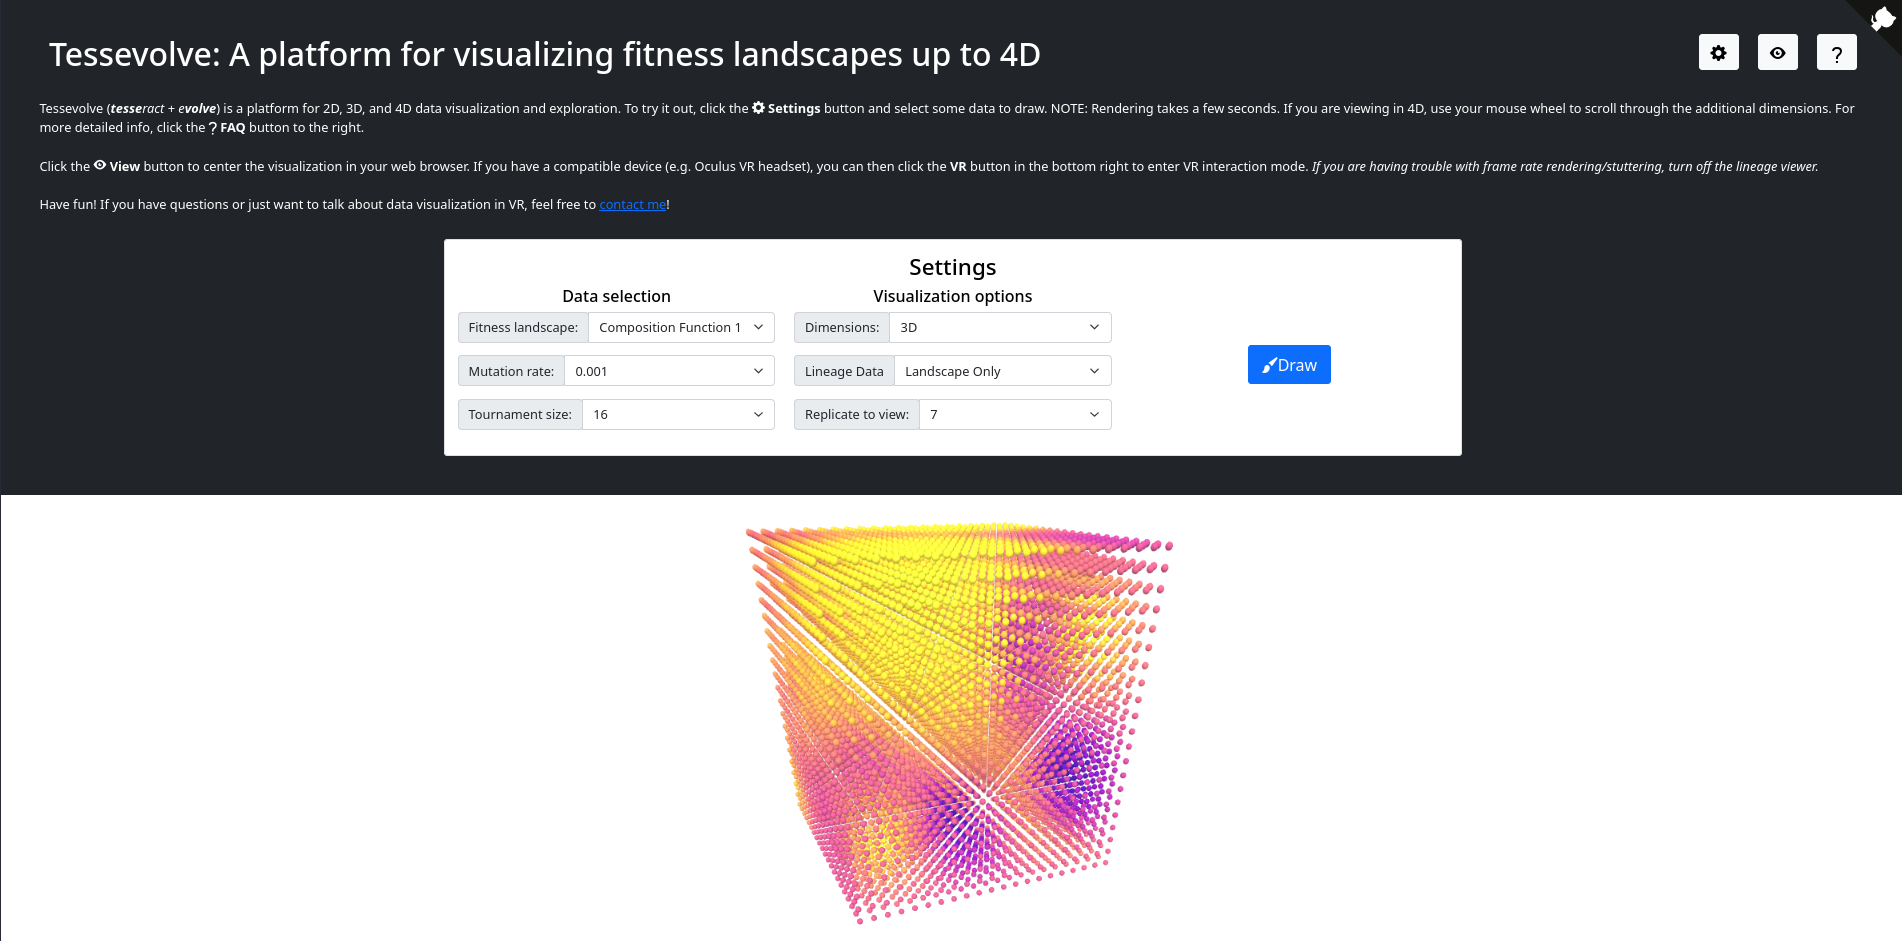
\includegraphics[width=\textwidth]{chapters/3-vr-viz/figs/tessevolve.png}}
    \caption{Tessevolve web interface. Changing the settings in the settings drop-down panel and clicking `Draw' allows users to load an updated landscape. The FAQ provided in the top right contains detailed information about the display. Drop-down menus allow users to select the combinations of parameters they are interested in seeing; the Draw button loads that configuration into the JavaScript DOM. The configuration of settings shown here is used in all other figures unless otherwise stated.}
    \label{fig:imp:tessevolve}
\end{figure*}


Tessevolve is available through any modern web browser at \url{https://alackles.github.io/tessevolve}.

The front-end interface for Tessevolve is a simple interactive web page (\autoref{fig:imp:tessevolve}). The top banner contains brief information about the site, displays for additional info, and a settings panel. Under the settings panel is an embedded A-Frame scene which can be adjusted to fill the screen or, in a VR headset, sent to VR mode. 

Under the hood, the site stores pre-processed landscape and lineage data for several evolutionary conditions and replicates. When users adjust the settings in the settings panel and click the Draw button to cue the site to reload, the embedded scene clears the old data and loads the new. 

The result is a 3D projection of the selected landscape. Users on the web version can navigate around the projection with the WASD or arrow keys and change viewing direction using the mouse; in VR, they can move with the left joystick or by walking around the space. 

\subsection{Dimension Comparisons}

Users can view the same landscape and its associated lineage in 2D, 3D, or 4D. Each dimension has its own unique design choices to help build intuition about extension into higher dimensions.

\subsubsection{2D Landscapes}

2D landscapes are displayed as a vertical grid of spheres in 3D space. Trait values are mapped to vertical and horizontal coordinates, while fitness is mapped to the Plasma color scheme (FIG). These landscapes are simple enough that they could be represented using the traditional relief map technique,  where fitness is used as a third dimension; see for example \autoref{fig:related-work:2dviz}. However, to keep visualization consistent across dimensions and maintain the analogy from 2D to 3D and 3D to 4D, 2D landscapes here are instead shown as if they were a single ``slice" of a 3D landscape. 

Lineage data is displayed as cubes connected by lines. Each cube represents the birth of a new \textit{taxon}---that is, in this case, a novel trait value. Cube positions represent trait values and color represents fitness; lines connect consecutive taxa. 

\subsubsection{3D Landscapes}

3D landscapes are displayed as an evenly-spaced mesh of spheres in 3D space. As in 2D, traits and fitness are mapped to position and color respectively in both landscapes and lineages. The only difference between the 2D and 3D landscape visualizations is the additional dimension.

\subsubsection{4D Landscapes}

4D landscapes required more complex design choices to account for the fourth dimension, which cannot be displayed concurrent with the other three. Here, the user sees one 3D ``slice" of the landscape at a time, and can move through the slices by scrolling. Each slice represents a different value for the fourth dimension, and fitness is computed based on the total trait values across all four dimensions. The result is that the spheres' positions remain fixed, while the colors change across the landscape to represent how fitness is changing over each slice. This representation was loosely inspired by Bosch's 4D toy-box application \citep{bosch_n_2020}.

Lineage data also adjusts depending on the current 3D slice. The connections between nodes are always displayed, but the colors of the nodes are only displayed when that node falls on the currently-viewed slice. Otherwise, nodes are greyed out and transparent to indicate that they are not present in this slice.
\section{Expert Feedback}
We solicited feedback from three domain experts whose primary disciplines were in three different fields in which evolutionary fitness landscapes are common: one in evolutionary and theoretical biology, one in machine learning and evolutionary computation, and one in digital evolution and artificial life. They were asked to rate the ability to use and interpret data in Tessevolve as easier, harder, or about the same as current methods they are familiar with, and then to provide open-ended responses about their experience with the platform. Expert feedback was generally positive, especially regarding interpretability across dimensions and the intuitive use of the visualization tool.  

\subsection{Ease of Interpretation}

Two of the three experts rated Tessevolve as \textit{easier to interpret} than current methods for both 3D and 4D data, with one pointing out that so few methods even exist for 3D and 4D data that they currently avoid attempting to visualize such data. These experts also provided qualitative feedback about the ease of interpretation:

\begin{displayquote}

\textbf{Expert 1:}  I had a hard time answering some of the questions [about comparative ease of use] since I don't generally try to visualize 3D or 4D fitness landscapes since I don't have tools to do so easily.

\textbf{Expert 2:} Overall I was pleasantly surprised by how easy it was to view both landscapes and lineages in 2D and 3D! I believe the 4D mode would become more useful as time goes on and you are better able to wrap your brain around it. That said, even with just a few moments I was able to see the effect of the fourth dimension on some landscapes, so it may not take long to build that intuition. 


\end{displayquote}


One expert found the 3D data harder to interpret than current methods, and was unsure about the interpretability of 4D data. However, their feedback on the tool indicated they were unable to find the explanation of positionality and color mappings provided on the website:

\begin{displayquote}

\textbf{Expert 3:} Moreover, I think you might add a line or two with the syntax of the visualisation; I am not a big expert in landscape visualisation, but I found it non-intuitive.

\end{displayquote}

This syntax was at the time provided in the FAQ, but based on this feedback we moved it to the front matter of the website.

All three experts found 2D data harder to interpret or about the same as current methods. This makes sense, as current methods such as topographical fitness landscapes are explicitly designed to handle 3D data, while Tessevolve explicitly chooses to sacrifice 2D interpretability in favor of improved ease of comparison to multiple dimensions. 

\subsection{Ease of Use}

Two of the experts agreed that the controls for Tessevolve were intuitive and that it ran well in the browser and in the Oculus headset:

\begin{displayquote}

\textbf{Expert 1:} I'm very impressed how well it runs in the browser and the controls were intuitive. 

\textbf{Expert 2:} I could definitely use this in my own work, as visualizing lineages in 3D is no easy task, even though it can really help build your understanding of the system. The VR support in particular is really useful for actually understanding the space in 3D.

\end{displayquote}

Expert 3 had some trouble rendering the 2D landscapes, but we and the other experts were unable to replicate this difficulty; they did not provide other comments related to ease of use.

\subsection{Constructive Feedback}

All three experts provided some constructive feedback on the visualization that we incorporated into our final design. 

As noted, one expert had trouble interpreting the landscape's design, and we attribute this to the fact that this information was in a pop-up menu in the FAQ. We therefore moved this information to the front of the page. We similarly moved information about the color scheme to the front page based on feedback from Expert 2 regarding uncertainty about whether the scheme transferred to the lineage data:

\begin{displayquote}

\textbf{Expert 2:} One thing I would suggest would be a guide to the color system for both the landscape and the lineage. It appears that the landscape shifts from purple to yellow as fitness increases, but the lineage colors are more difficult to deduce. 

\end{displayquote}

Given that experts generally found Tessevolve easier to use for multidimensional data, and critical comments were related to the front-facing interface rather than the visualization itself, this initial round of expert feedback indicates Tessevolve can be an effective tool for 3D and 4D landscape data visualization.
\section{Discussion}
In addition to the expert comments on ease of use and interpretability, we found that Tessevolve provides novel insight about which landscape dynamics may change as dimensions increase, and which may remain constant. In particular, we found that Tessevolve allowed us to see that, for the landscapes used here, \textit{landscape ruggedness} remains relatively unchanged as dimensions increase, but the ability to perform \textit{valley-crossing} greatly increases.

\subsection{Landscape Ruggedness}

Landscape ruggedness is a measure of how quickly fitness changes across a landscape. In smooth landscapes, points that are close together in evolutionary space will have similar fitness values. However, in very rugged landscapes, close points could have very different fitness values. 

\begin{figure}
    \centering
    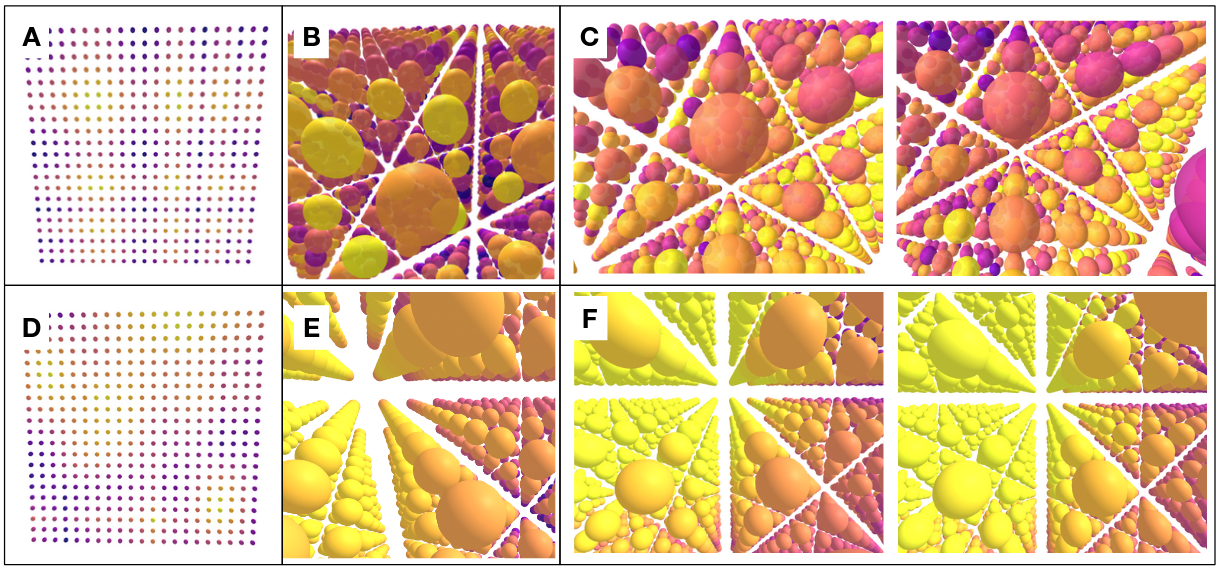
\includegraphics[width=0.5\textwidth]{chapters/3-vr-viz/figs/rugged.png}
    \caption{Ruggedness in Vincent (top) and Composite Fitness 1 (bottom) landscape. Note how properties of ruggedness transfer across dimensions. (A,D) 2-Dimensional landscape. (B,E) 3-Dimensional landscape. (C,F) Adjacent slices of 4-Dimensional landscape. }
    \label{fig:disc:rugged}
\end{figure}

The visual, color-based display of Tessevolve allowed us to see that landscapes which are rugged in lower dimensions also tend to be rugged in higher dimensions (\autoref{fig:disc:rugged}). This is mathematically unsurprising but previously difficult to visually demonstrate. Here, a smooth color gradient either across space (for 2D or 3D) or on scrolling (for 4D) easily maps to the concept of a smooth fitness gradient; similarly, colors that change very rapidly for adjacent spheres or slices are visually easy to notice and therefore easy to draw intuition about. This visual depiction of landscape ruggedness across dimensions helps reinforce intuition about how similar in fitness two similar trait states might be in higher-dimensional landscapes, even when we only have lower dimensional analogues. 

\subsection{Valley-Crossing in 2D vs. 3D vs. 4D}

\begin{figure}
    \centering
    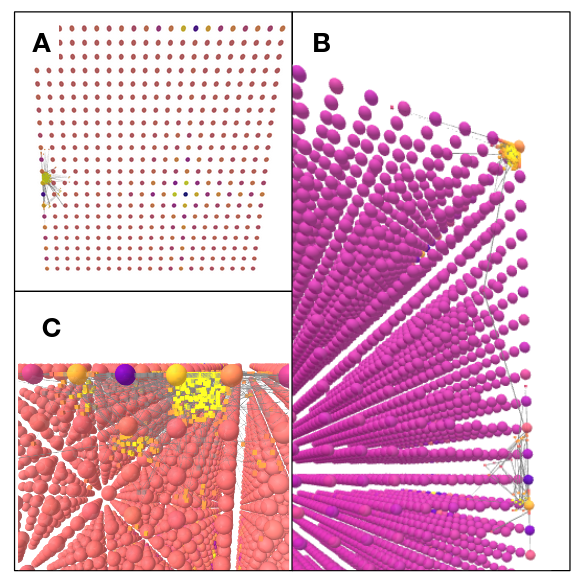
\includegraphics[width=0.5\textwidth]{chapters/3-vr-viz/figs/valley.png}
    \caption{Representative valley-crossing dynamics in 2D, 3D, and 4D. In each case, the Shubert function is the underlying evolutionary landscape, and populations mutate every generation with a standard deviation of 0.0001 and tournament size 16. The only difference in each is case is the number of dimensions. (A) 2D lineage where no valley-crossing occurs. (B) 3D lineage where valley-crossing occurs once across a large valley. (C) 4D lineage where the lineage stays primarily near one peak, but hops around nearby peaks frequently. }
    \label{fig:disc:valleys}
\end{figure}

In contrast to landscape ruggedness, one landscape feature that changed dramatically across landscapes was ease of landscape traversal and particularly ease of valley-crossing. As noted earlier, valley crossing is of particular interest because it helps to explain how populations transition from local optima to global optima. Here, the ability to visualize a lineage evolving across both a 2D and 3D landscape in multiple replicates demonstrates a quantitative difference in landscape traversal between replicates. For one set of parameters displayed in \autoref{fig:disc:valleys}, valley crossings from optimum to optimum occurred in 0 out of 10 replicates, while in 3D landscapes, they occurred in 8 out of 10 replicates. In all eight of these transitions, there was only a single valley crossing observed in the 1000 generations, and these peaks tended to be reasonably far apart (approximately half the distance of the entire landscape).

In 4D, however, rather than a single valley crossing from a one local optima to another, lineages tended to ``bounce" around closer peaks  multiple times across their evolutionary history. While there were some ``major" valley crossing as in 3D, the dominant dynamic was these more ``minor" crossings. 

The dynamics underlying these major vs.~minor valley crossings are not obvious from the visualization, nor are they intended to be; however, this visualization provides the insight that examining these large or small crossings might change across dimensions. 
\section{Conclusion}
Here we introduced Tessevolve, a platform for visualizing fitness landscapes in 2D, 3D, and 4D. The concept was inspired by a lack of existing tools for qualitatively understanding how fitness landscapes change as additional dimensions are added. It was designed to be intuitive, customizable, and extensible. Based on expert feedback, we conclude that Tessevolve is an effective and easy-to-use tool for gaining a stronger intuitive understanding of complex fitness landscapes.

Experts found that when viewing 3D and 4D landscapes, Tessevolve was generally easier to use and interpret than existing platforms they are familiar with. They also reported that the landscape visualization was easy to interpret, even when given minimal information beyond the built-in interface. We incorporated their feedback about adding a clearer and more apparent key to the visualization components to improve Tessevolve's usability and overall design. 

In the future, Tessevolve could incorporate additional sources of information for additional dimensionality. In particular, leveraging the audio input capabilities of VR headsets could allow us to expand into more dimensions, or replace color as a fitness indicator to make the visualization more accessible to blind or low-vision researchers.

Another improvement we are considering, which may be particularly helpful for large and complex landscapes, would be to add a mode inspired by the holey fitness landscape concept (see Domain Background). In this mode, the user would enter a fitness threshold that they were interested in viewing. Tessevolve would then render 3D shapes representing the regions of the search space with fitnesses below that threshold. This approach would allow the user to quickly build intuition about a larger region of the search space, at the cost of reducing the resolution at which fitness is displayed.

The generally positive feedback from domain experts indicates that Tessevolve is a valuable new tool for evolutionary biology and computational evolution. While the number of dimensions Tessevolve can display is still limited, the ability to compare properties across dimensions allows for insight into how dimensionality affects evolutionary dynamics. In particular, Tessevolve reveals the ways landscape ruggedness and landscape traversal intersect with the number of landscape dimensions. It is our hope that Tessevolve, and other VR-based visualizations, can continue to push the boundaries of human ability to comprehend complex fitness landscapes. It has been decades since the problems with building intuition from low-dimensional visual fitness landscape metaphors were first pointed out. Perhaps now we can finally begin building a better visual metaphor.
\section{Acknowledgements}
The authors sincerely thank artist Kathleen (Katie) Gleason for her contribution to the figures for this paper. 
We thank Charles Ofria, Clifford Bohm, and Vincent Ragusa for helpful comments on early versions of Tessevolve. 
This material is based in part upon work supported by a National Science Foundation Graduate Research Fellowship to A.A. and by the National Science Foundation under Cooperative Agreement No. DBI-0939454. 
Any opinions, findings, and conclusions or recommendations expressed in this material are those of the author(s) and do not necessarily reflect the views of the National Science Foundation. 
This work is also supported by Michigan State University.
Michigan State University, where this work was conducted, occupies the ancestral, traditional, and contemporary Lands of the Anishinaabeg–Three Fires Confederacy of Ojibwe, Odawa, and Potawatomi peoples. 
The University resides on Land ceded in the 1819 Treaty of Saginaw.
\chapter{Conclusion}
\label{ch:conclusion}

\section{Introduction}

In this dissertation, I introduced three new methods and metrics for investigating connectivity in evolvable systems at the genotype, phenotype, and landscape levels. 
Each of these new methods provided insight into their respective systems that existing techniques obfuscated or failed to detect. 
Together, these new tools represent both quantitative and qualitative improvements towards our understanding of key evolutionary processes.
\section{Contributions}

In summary, this dissertation makes the following contributions:

\begin{itemize}
    \item In \textbf{Chapter \ref{ch:re}}, I developed a rank-based metric for measuring genome connectivity that does not rely on underlying assumptions of baseline interaction. This model was able to correctly identify when loci were non-interactive in a case where existing metrics failed. Rank epistasis therefore allows us to better detect when epistasis is present, leading to more accurate understanding of interactivity within genomes. 
    \item In \textbf{Chapter \ref{ch:chm}}, we introduced the comparative hybrid method, an analytic tool for comparing computational cognitive structures. Using this method, we showed that connectivity and discretization are important components in the evolution of associative learning. These results demonstrate the value of a piecewise approach to analysis of evolving systems. 
    \item In \textbf{Chapter \ref{ch:vr-viz}}, I describe Tessevolve, a platform for visualizing and exploring fitness landscapes in up to four dimensions. Tessevolve expands our current ability to view and manipulate landscapes visually and allows us to view how patterns of ruggedness and mutational landscape connectivity change across dimensions. This platform represents a novel approach to the visualization of 3D and 4D fitness landscapes. 
\end{itemize}

As a whole, this dissertation contributes to our understanding of connected systems across multiple scales. it provides new tools and sets up a framework for thinking about connected systems in a digital evolution context, and lays groundwork for future studies on the computational study of evolvable networks and systems.


\section{Future Directions}

I have so far provided overviews of three distinct metrics for evolutionary phenomena as well as representative examples of phenomena studied with each metric. These metrics dealt primarily with investigating the underlying connected structures of their respective evolvable systems. Here I present two branches for future directions to further investigate these systems: introducing information theory to current methods, and expanding our ability to interface with our data with novel metrics.

\subsection{Information-theoretic extensions to existing metrics}

The metrics introduced here have produced promising results for studying connectivity in evolvable systems. Further building upon these metrics would allow us to work towards a more complete picture of the underlying physical and mathematical constraints on our systems of interest. In particular, the quantitative and broadly applicable nature of information theory is a promising direction for metric expansion.


\subsubsection{Rank epistasis on information-theoretic networks}

The effect of epistasis on genotype structure can be quantified using information theory via \textit{statistical epistasis networks} \citep{moore_flexible_2006, mckinney_six_2012}.
In essence, epistatic loci or genes are nodes on the network, while edges represent interaction. 
These edges can be derived from the rank epistasis process by tracking which genotype rankings are altered for each double-mutant. 

Then, information theory as developed on networks can be applied to these epistatic networks; in particular, those information-theoretic metrics which were developed to quantify evolutionary networks \citep{sole_information_2004, adami_information_2011, carpi_analyzing_2011}. By viewing epistatic interactions as a network, we effectively get all the tools of network information theorry to apply to epistasis.

\subsubsection{Adding informational network flow to the Comparative Hybrid Method}

In introducing the Comparative Hybrid Method, I discussed how the method gives a high-level, qualitative understanding of the impact of structure on function. 
However, quantifying this impact is also essential for deeper study of connectivity and constraint within computational architectures.
One direction for such quantification is analysis of informational network flow, or how information traverses the computational cognitive networks to create output.
Such a technique has been used in to investigate cognitive networks in the past and could readily be applied to comparative hybrid structures in the future \citep{bohm_information_2022}. 
By analyzing the informational network flow of hybrids versus their canonical counterparts, we could understand how changing structure on the phenotypic level changes information at the genotypic level, expanding our understanding of their mapping.

\subsection{Expanding our ability to interface with biological data}

In the past, our ability to interface with data has been limited to charts, tables, formulae, and figures--all of which are two-dimensional. However, biology moves and lives in three dimensions, and data about biology exists in many more dimensions than that. Therefore, leveraging emerging technology to expand our spatial and dimensional understanding of connections between system components will be essential to future breakthroughs in evolutionary theory.

\subsubsection{Creating audioscapes in VR}

The 3D visual landscape provided by virtual reality is a powerful tool for exploring fitness landscapes. 
An immediate next step in this research is to leverage the immersive sound capabilities of VR headsets to map landscape information to audio output. 
Such data sonification has been used in astrophysics to reveal patterns not obvious from mathematical or visual models alone \citep{gibney_how_2020}.
By leveraging audio as well as visual input, we can further expand the number of available dimensions in our audiovisual model.
Sonfiication would also expand the use case for these VR models to scientists who are blind/low-vision, colorblind, or otherwise may benefit from audio data interpretation over visual.

\subsubsection{Spatial models of genome structure}

Finally, in the next few years of my research I hope to merge the development of new frameworks with novel 3D data interfacing and develop multidimensional spatial models of genomes and genetic networks.
Genome models in artificial life and evolutionary computation are typically one-dimensional (i.e.~vectors), but biological genomes evolve and interact in three-dimensional space. 
Understanding how genomes move in 3D space is essential to understanding complex processes such as gene regulation and modification \citep{mendizabal_epigenetics_2014, sotelo-silveira_entering_2018}.
Therefore, I would create novel models of genetic structures and networks to investigate how evolutionary forces are shaped by space and dimensionality.
Such modeling could range from comparing evolutionary dynamics of digital genomes of different dimensionality to creating entirely new evolving genome models within 3D physics emulators. 
These spatial models could hopefully provide insight into what it is like to be where science can only go in theory: inside the genome itself.
\end{raggedbottom}

%%%  Appendices, if necessary:

% \begin{centering}
% \vfill
% \appendix{APPENDICES}                      %Make sure the names in
% \addcontentsline{toc}{chapter}{APPENDICES} %brackets match
% \vfill
% \end{centering}
% \newpage
% \input{appendix/appendix} %====Put you Appendix text here
% \clearpage


%\pagenumbering{gobble}% Remove page numbers (and reset to 1)
%%%  Bibliography:
\addcontentsline{toc}{chapter}{BIBLIOGRAPHY}

\newpage
\vspace*{\fill}
\begin{center}
BIBLIOGRAPHY
\vspace*{\fill}
\end{center}

\newpage
\begin{singlespace}
\bibliographystyle{apalike}% your bst file here
\bibliography{references} %your bib file here
\end{singlespace}
\end{doublespace}
\end{document}